\documentclass[11pt,a4paper]{article}

\usepackage[margin=2.5cm]{geometry}
\usepackage{amsmath,amssymb}
\usepackage{graphicx}
\usepackage{booktabs}
\usepackage{caption}
\usepackage[numbers,sort&compress]{natbib}
\usepackage{xcolor}
\definecolor{linkcol}{RGB}{25,60,130}
\usepackage[colorlinks=true,linkcolor=linkcol,citecolor=linkcol,urlcolor=linkcol]{hyperref}

\captionsetup{font=small,labelfont=bf}
\setlength{\emergencystretch}{3em}
\sloppy
% let floats pack more tightly, so the paper does not run to float pages
\renewcommand{\topfraction}{0.92}
\renewcommand{\bottomfraction}{0.85}
\renewcommand{\textfraction}{0.06}
\renewcommand{\floatpagefraction}{0.85}
\setlength{\floatsep}{10pt plus 2pt minus 2pt}
\setlength{\textfloatsep}{12pt plus 2pt minus 3pt}
\setlength{\intextsep}{10pt plus 2pt minus 2pt}
\graphicspath{{figures/}}

\newcommand{\um}{\ensuremath{\,\mu\mathrm{m}}}
\newcommand{\mm}{\ensuremath{\,\mathrm{mm}}}
\newcommand{\qop}{\ensuremath{\mathrm{qop}}}

% ---------------------------------------------------------------------------
\title{A label-free surrogate for track extrapolation in LHCb:\\
the discrete-time physics-informed construction measured\\
against the scheme it solves}

\author{George William Scriven\thanks{george.w.scriven@gmail.com}\\[2pt]
\normalsize Maastricht University, Maastricht, The Netherlands\\
\normalsize Hasselt University, Hasselt, Belgium\\
\normalsize Nikhef, Amsterdam, The Netherlands}

\date{\today}

\begin{document}
\maketitle

\begin{abstract}
Track reconstruction in LHCb calls an extrapolator, the routine that transports
a five-component track state from one detector plane to another through the
spectrometer magnet, millions of times a second. The standard implementation
integrates the equation of motion numerically, at a cost that is accurate but
neither fixed nor predictable. I build a surrogate for the field-propagation
part of that routine from the discrete-time construction of Raissi, Perdikaris
and Karniadakis, in which a neural network emits all internal stage states of an
implicit Runge--Kutta step at once and is trained only by the requirement that
those states reconstruct the starting state. No label enters the loss anywhere.
The training population is harvested from an official LHCb simulation sample,
$323{,}533$ extrapolation legs of four geometrical kinds, split by particle.
Every result is quoted against three fixed comparators: the same
Gauss--Legendre scheme solved exactly by a root-finder, a supervised twin
trained on Runge--Kutta labels under an identical protocol, and a straight line
that ignores the magnet. On one frozen $5178\mm$ crossing of the magnet the
label-free network reaches a median endpoint error of $115\um$ at four layers of
$200$ units, three and a half orders of magnitude below the straight line and,
at that size, $12$ percent better than its own supervised twin. Where the
discretisation is the limiting factor the network reproduces the scheme's own
error to within $0.1$ and $0.6$ percent at two and four stages, which is the
cleanest available demonstration that the loss does what it claims. Where the
network is the limiting factor the shortfall is optimisation and not capacity:
over $96$ converged runs spanning $12$ architectures and $10$ seeds, the
Spearman rank correlation between final training loss and held-out endpoint
error is $+0.965$. Trained on the reversed magnet polarity, for which no
labelled sample exists anywhere in the project, the same construction reaches
the same floor, $229\um$ against $222\um$, and sits the same distance above that
polarity's own ceiling. Generalising to one network for every kind of step, with
the start plane and the step length as inputs, first cost a factor $14$ on the
magnet crossing and left the network fifty times worse than a straight line on
the short steps. Changing what the network outputs, from the absolute state to
the deviation from straight-line propagation normalised by a per-leg bending
integral built from the inputs alone, improved the two short leg types by
factors of $92$ and $190$ and moved both from thirty to fifty times worse than
ignoring the magnet to two to four times better than it, at $2.1\um$ on the
whole test split against $16.1\um$ for a straight line. Walked along real
particle paths the redesigned network is four to thirteen times more accurate
than its predecessor at every chain length. The remaining constraint is the
magnet crossing itself inside the shared network, $1026\um$ against a $46\um$
ceiling, which the redesign improved by only a factor $2.5$ and which now
dominates both the one-step and the chained error. The evidence base is
$232$ training runs.
\end{abstract}

\tableofcontents

% ===========================================================================
\section{Introduction}
\label{sec:intro}

LHCb is one of the four large experiments at the Large Hadron Collider at CERN,
rebuilt for the current data-taking period as a fully software-triggered
spectrometer~\cite{lhcb2024upgrade}. Two beams of protons are brought into
collision at its centre roughly thirty million times a second. Each collision
sprays out charged particles, and the detector's job is to work out which
particles were produced and where they came from. It does this by placing layers
of position-sensitive silicon and scintillating fibre along the beam direction,
so that a particle passing through leaves a series of measured points, called
hits. A \textbf{track} is the reconstructed path of one charged particle through
the detector, fitted to those hits.

Between the layers near the collision point and the layers further downstream
sits a large dipole magnet. Its field is roughly vertical and peaks at about
$1.05$ tesla around $4.7$ m downstream of the collision point.\footnote{I
write distances in millimetres throughout, because that is what the
reconstruction software does, and I have never once regretted matching the
code's units rather than the reader's intuition.} A charged particle passing
through a magnetic field is deflected, and the amount of deflection depends on
its momentum: fast particles are barely bent, slow particles are bent a great
deal. The magnet is therefore the instrument that measures momentum. It is also
the reason the geometry of a track is not a straight line, and the reason this
paper exists.

Throughout I work in a coordinate system in which $z$ runs along the beam
direction, $x$ is horizontal and transverse to the beam, and $y$ is vertical.
Because LHCb detects particles that go forward at small angles to the beam,
every particle of interest moves monotonically in $z$, and it is convenient to
describe a track not as a function of time but as a function of $z$.

A \textbf{track state} is the complete description of a track at one value of
$z$. It is a list of five numbers,
%
\begin{equation}
  S = (x,\ y,\ t_x,\ t_y,\ \qop),
  \label{eq:state}
\end{equation}
%
where $x$ and $y$ are the transverse position of the track at that $z$ in
millimetres; $t_x = \mathrm{d}x/\mathrm{d}z$ and $t_y = \mathrm{d}y/\mathrm{d}z$
are the local slopes, dimensionless; and the fifth component encodes the
particle's charge $q$, in units of the proton charge, divided by its momentum
$p$. I use the convention of Allen, the GPU high-level trigger of
LHCb~\cite{aaij2020}, in which that component is stored as
%
\begin{equation}
  \qop = 0.299792458\,\frac{q}{p[\mathrm{GeV}]}.
  \label{eq:qop}
\end{equation}
%
Five numbers suffice, because once you know where a particle is, which way it is
pointing, and its charge-to-momentum ratio, the magnetic field determines the
rest of its path.

An \textbf{extrapolator} is the piece of software that takes a track state at
one plane $z_0$ and returns the track state at another plane $z_1$. That is the
whole of its job, and it is used constantly: when a track fit walks along a
candidate track from measurement to measurement; when the reconstruction asks
whether a track found in front of the magnet and a track found behind it are the
same particle; and when a vertex fit asks where several tracks came closest to
one another, which requires each of them to be transported back towards the
collision point. In the high-level trigger this happens millions of times per
second, on every event, inside the time budget that decides whether the event is
written to disk at all.

The standard extrapolator does this by numerical integration: it steps along $z$
in small increments, evaluating the magnetic field at each step. It is accurate
and it is not cheap. A method that could take a single large step, at comparable
accuracy, using a fixed and predictable amount of arithmetic, would be worth
having twice over. It would be faster, and a fixed arithmetic cost is much
easier to schedule on the parallel hardware the trigger runs on than a loop
whose trip count depends on the track.

That is the surrogate this programme is trying to build. The restriction I work
under throughout is that the surrogate replaces \textbf{field propagation only}.
Real particles also scatter off the detector material and lose energy to it;
those effects stay with the existing extrapolator, and none of the numbers in
this paper include them.

\subsection{The label-free idea}

The technique I use is the discrete-time construction of Raissi, Perdikaris and
Karniadakis~\cite{raissi2019}, referred to throughout as \emph{the source work}.
Its distinguishing feature, and the reason I chose it over the more familiar
supervised alternative, is that it needs \textbf{no labels}. The network is
never shown a correct answer. It is trained only by being required to satisfy
the algebra of an implicit Runge--Kutta step, which is arithmetic, together with
the magnetic field, which is a measured map. Section~\ref{sec:construction}
states the construction exactly.

If that works it is valuable for a reason beyond elegance. Producing labels for
a surrogate of this kind means running the reference integrator over a large
sample, and it has to be redone whenever the field map, the detector geometry or
the state conventions change. A loss that never touches a label is immune to all
three. The strongest version of that claim, and the one I test in
Section~\ref{sec:magnetup}, is that the method should work on a configuration
for which no labelled sample has ever been produced.

\subsection{The two questions}

I set two questions at the start of the programme and stated in advance what
each would mean, so that the answers could not drift to meet the results.

\begin{enumerate}
  \item \textbf{Does it work?} By this I mean: does the label-free training
  converge at all; does the trained network reach the accuracy that the
  numerical scheme it is being trained against can itself reach; and where the
  network falls short of that, is the shortfall understood? A yes requires the
  training to be stable, the network's error to sit on the scheme's own error in
  the regime where the scheme is the limiting factor, and the remaining gap in
  the other regime to be attributable to something identified rather than left
  as a mystery.

  \item \textbf{Can it be used?} By this I mean: can one trained network be
  pointed at an arbitrary extrapolation step, of arbitrary length, starting
  anywhere, and be used repeatedly along a particle's path, at an accuracy that
  is better than doing nothing? A yes requires a single network to serve every
  kind of step, to beat the trivial baseline of ignoring the magnet on every
  kind of step, and to have an error that does not compound uncontrollably when
  the network is applied to its own output.
\end{enumerate}

Question 1 is about the method. Question 2 is about the product. They are
separable, and, as Section~\ref{sec:results} shows, they came out differently.

\subsection{The relation to the van der Pol study}

Before any of this ran on LHCb data I rebuilt both of the source work's
constructions on a completely controlled test problem, the van der Pol
oscillator, and measured them against a reference solution whose own error is
negligible. That study is a companion to this one~\cite{scriven2026vdp}. Its
role here is not decorative: every design choice in the present work that could
have been argued about was settled there first, on a problem small enough to
measure exhaustively. Section~\ref{sec:papers} lists which findings transferred
and how. The short version is that the discrete-time construction was shown, on
the oscillator, to be limited by the optimiser rather than by network capacity,
to be sensitive to the training seed in a way that a validation chain can
diagnose, and to land within a small factor of perfect-label training at zero
label cost. All three of those statements reappear in this paper, measured
independently on a five-dimensional non-autonomous system with a field that is
not an analytic function.

\subsection{Road map}

Section~\ref{sec:papers} is a related-work section: what the source work
actually contains, what the van der Pol study established, and what the recent
literature on the failure modes of physics-informed training says about the
construction I have deliberately not used here.
Section~\ref{sec:theory} derives the method from the equation of motion up,
defines the loss exactly as it is implemented, and defines the three
comparators, the metrics, the training protocol and the output
parameterisation. Section~\ref{sec:data} describes the data and the shared
machinery. Section~\ref{sec:results} reports each experiment in turn and then
assembles the verdict. Section~\ref{sec:discussion} reads that verdict against
the two questions and lists the caveats honestly.
Section~\ref{sec:outlook} says what happens next. Appendix~\ref{app:prov}
carries the provenance.

% ===========================================================================
\section{The papers we build on}
\label{sec:papers}

\subsection{The source work, and its two constructions}

Raissi, Perdikaris and Karniadakis~\cite{raissi2019} introduced physics-informed
neural networks: networks trained on a loss that contains the differential
equation itself, evaluated on the network's own output, in place of or in
addition to measured data. The paper contains two distinct constructions, and
the distinction matters a great deal for what follows.

The \textbf{continuous-time} construction, the paper's Section 3.1, makes the
network \emph{be} the solution. Time, and space too for a partial differential
equation, go in; the solution value comes out; the residual of the equation is
enforced by automatic differentiation at sampled points of the domain. It is the
form most people mean by the phrase.

The \textbf{discrete-time} construction, the paper's Section 3.2, is different
in kind. The network does not represent a solution over a domain. It represents
one step of an implicit Runge--Kutta scheme: given a state, it emits all the
internal stage states of the step at once, and the algebra of the step supplies
the supervision. The source work demonstrated it on Burgers' equation and on the
Allen--Cahn equation, in both cases taking a single very large time step with a
high-stage Gauss--Legendre scheme, and reported that the construction tolerates
step sizes far beyond what the same scheme would be stable at if solved
conventionally. Its stated limitation is that the network is tied to one
starting condition and one step: the paper trains a network for a specific
initial state and a specific $\Delta t$, and says nothing about reuse. That
limitation is exactly what Section~\ref{sec:general} attacks, by making the
starting state, the start plane and the step length inputs.

I use the discrete-time construction throughout this paper. The continuous-time
one is deferred, and Section~\ref{sec:outlook} says under what conditions it
would be opened. The reason for deferring it is not taste. It has no fixed
arithmetic cost per step, which is the property the trigger wants; it imposes a
much weaker constraint per training point; and, as the next two subsections
record, it has a documented failure mode on long horizons that the discrete-time
construction structurally cannot have, because a discrete-time network is never
asked to represent a trajectory over an interval at all.

\subsection{What the van der Pol study established}

The companion study~\cite{scriven2026vdp} rebuilt both constructions on the van
der Pol oscillator under identical optimiser discipline. Four of its findings
shaped this programme directly.

\textbf{The capacity floor is an optimisation floor.} A $135$-run architecture
sweep on the discrete-time construction found an endpoint error floor that
larger networks did not remove, and identified it by measuring the rank
correlation between the final training loss and the held-out one-step error:
$+0.974$. Every architecture and every seed lay on one loss-error band. The
conclusion was that a wider network helps only because the optimiser gets
further down on it, not because the narrower network could not represent the
answer. Section~\ref{sec:size} repeats that measurement on the magnet crossing
and gets $+0.965$, which is the same statement about a very different system.

\textbf{The seed is a real degree of freedom, and the chain selects it.}
Long-horizon quality on the oscillator was decided by the training seed, was
measurable on a validation chain, and transferred to held-out starts. The
protocol that came out of it, train ten seeds, chain each to the target horizon
on validation data, keep the best, is the protocol
Section~\ref{sec:general} uses on real particle paths.

\textbf{Supervision is the right control, not the right method.} The oscillator
study ran a matched data-supervised twin: same network, same initialisation,
same optimiser, same budget, physics loss swapped for mean squared error against
the reference. The equation-trained network landed within a factor $2.1$ of
perfect-label training at zero reference-data cost. That twin is reproduced here
for every experiment, and Section~\ref{sec:size} reports the one regime where
the label-free loss overtakes it.

\textbf{Chaining a reusable one-step map beats one large step.} On the
oscillator, generalising the discrete-time network so that its input is the
starting state itself, and then applying it repeatedly, beat the source work's
single-large-step mode by a factor $10$ at the largest feasible step. That is
the design used here from the outset: the network is a one-step map, and
Section~\ref{sec:general} walks it.

\subsection{The stability line, and why it argues for the discrete-time column}
\label{sec:stability}

The continuous-time construction has a failure mode that is now well
characterised, and understanding it is the main reason the parked column stays
parked. I summarise the three papers because they bear directly on what would
happen if the LHCb work opened that line.

Rohrhofer, Posch, G\"o\ss{}nitzer and Geiger~\cite{rohrhofer2023} observe that
if the network output is a constant equal to a fixed point $y^\ast$ of the flow,
so that $f(y^\ast) = 0$, then its time derivative is zero and the residual is
exactly zero at every collocation point, wherever those points sit. Fixed points
are therefore global minima of the residual term, with basins that grow with the
horizon, and only the initial-condition term prefers the true solution. They
measure success falling monotonically with horizon and with proximity of the
start to a fixed point, and report that larger networks repair nothing,
concluding that the difficulty is bound to optimisation complexity rather than
to expressive power. They propose no remedy.

Wang, Koohy, Lu and Perdikaris~\cite{wang2026pseudo} sharpen this into a
statement about the whole family of spurious minimisers. For any fixed
collocation set there exists a candidate that follows the true solution near
every collocation point before some time $t_0$, follows a different solution of
the same equation after it, and hides the hand-over in the gaps between
collocation points, so that its empirical residual is \emph{exactly} zero. The
fixed point is only the cheapest member of that family. Their remedy is
pseudo-time stepping with collocation resampling, which penalises change from
the previous iterate and thereby amplifies the hidden transition layer.
Babic, Rohrhofer and Geiger~\cite{babic2025} instead propose a regulariser that
penalises a candidate for sitting still inside a locally unstable region, a
product of the positive real parts of the Jacobian eigenvalues at the network's
output and a Gaussian in the network's own speed, inert on any moving candidate
by construction, and demonstrate it on van der Pol to about two periods.

The van der Pol study measured all three. The finding that matters here is the
ordering: the regulariser turns parking at the fixed point into a different
member of the same family, a flow-following splice, and only pseudo-time
stepping prices the whole family rather than one member of it. Across $240$
converged runs, pseudo-time stepping was the only intervention that worked past
two periods.

None of this applies to the discrete-time construction as such. A discrete-time
network is asked for the stage states of one step, and the reconstruction
residual of Section~\ref{sec:construction} is not zero for a constant output:
the stage equations tie every output to the known starting state, which enters
the loss as data. There is no interval over which a hand-over can be hidden and
no free phase. That structural difference, rather than any measured comparison
on LHCb data, is why the discrete-time column was opened first.

\subsection{Gauss--Legendre collocation}

The numerical scheme underneath everything here is the Gauss--Legendre family of
implicit Runge--Kutta methods, whose classical theory is set out by Hairer and
Wanner~\cite{hairer1996}. Two of its properties are load-bearing. A $q$-stage
member has formal order $2q$, the maximum attainable by any $q$-stage
Runge--Kutta method, which is what makes it the right family for a method that
intends to take very few, very large steps. And the family is equivalent to
polynomial collocation: the $q$-stage scheme is exactly the polynomial of degree
$q$ through the step that satisfies the differential equation at the $q$ node
positions. Section~\ref{sec:irk} uses the second property as the mental picture
throughout.

% ===========================================================================
\section{Theory}
\label{sec:theory}

This section builds the method from the equation of motion up. I write down the
differential equation that governs a track in $z$ and say where each term comes
from; explain what makes a Runge--Kutta method implicit and why the
Gauss--Legendre family is the natural choice; describe the construction that
turns that scheme into a training objective with no labels; define the loss and
its scales; define the three comparators and the metrics; state the training
protocol and the fiducial requirement; and finally define the output
parameterisation that Section~\ref{sec:residual} tests.

\subsection{The equation of motion in \texorpdfstring{$z$}{z}}
\label{sec:eom}

A charged particle in a magnetic field $\mathbf{B}$ feels the Lorentz force
$q\,\mathbf{v} \times \mathbf{B}$. Rewriting Newton's second law with $z$ rather
than time as the independent variable, and expressing the result in the state
variables of Eq.~\eqref{eq:state}, gives the system that
\texttt{\_shared/reference.py} implements:
%
\begin{align}
  \frac{\mathrm{d}x}{\mathrm{d}z} &= t_x,
  &\frac{\mathrm{d}y}{\mathrm{d}z} &= t_y,
  \label{eq:eom1}\\[4pt]
  \frac{\mathrm{d}t_x}{\mathrm{d}z}
    &= \kappa\,\qop\,N\left[t_x t_y B_x - (1 + t_x^2) B_y + t_y B_z\right],
  \label{eq:eom2}\\[2pt]
  \frac{\mathrm{d}t_y}{\mathrm{d}z}
    &= \kappa\,\qop\,N\left[(1 + t_y^2) B_x - t_x t_y B_y - t_x B_z\right],
  \label{eq:eom3}\\[2pt]
  \frac{\mathrm{d}\,\qop}{\mathrm{d}z} &= 0,
  \label{eq:eom4}
\end{align}
%
where $\kappa = 10^{-3}$ is the unit conversion constant that goes with the
Allen $\qop$ convention of Eq.~\eqref{eq:qop};
$N = \sqrt{1 + t_x^2 + t_y^2}$ is the ratio of path length to $z$ length, which
appears because the force acts along the path while we differentiate along $z$;
and $B_x$, $B_y$, $B_z$ are the three components of the field in tesla,
evaluated at the point $(x, y, z)$ the particle currently occupies.

Three properties of this system matter for everything that follows.

\begin{itemize}
  \item \textbf{It is non-autonomous.} The right-hand side depends on $z$
  explicitly, through the field. This is unlike the textbook test problems on
  which the technique was originally demonstrated, where the right-hand side
  depends only on the state.
  \item \textbf{$\qop$ is conserved}, by Eq.~\eqref{eq:eom4}. A magnetic field
  does no work, so restricting the surrogate to field propagation makes the
  momentum an input that is carried through unchanged. Only four components are
  ever predicted.
  \item \textbf{The field is not an analytic function.} It is a measured map,
  stored on a grid, and Section~\ref{sec:floor} shows that this sets the ceiling
  on the whole exercise.
\end{itemize}

\emph{Analogy.} Equations~\eqref{eq:eom1} to \eqref{eq:eom3} say the same thing
as a description of a car on a road: the position changes at a rate given by the
current heading, and the heading changes at a rate given by how hard the
steering wheel is turned. The magnetic field is the steering wheel, and $\qop$
is how strongly the car responds to it. A heavy, fast car, meaning high momentum
and small $\qop$, barely turns; a light, slow one turns sharply.

\emph{Worked micro-example.} Take a particle with $p = 10$ GeV and charge $+1$,
so $\qop = 0.0300$ by Eq.~\eqref{eq:qop}. Take it travelling nearly along the
beam, $t_x = t_y = 0$, so $N = 1$, through a field of $B_y = -1.0$ T with
$B_x = B_z = 0$. Then Eq.~\eqref{eq:eom2} gives
$\mathrm{d}t_x/\mathrm{d}z = \kappa\,\qop\,(-1)\,B_y
 = 10^{-3} \times 0.0300 \times 1.0 = 3.0 \times 10^{-5}$ per millimetre. Over
the $5178\mm$ crossing of the magnet studied here, and treating the field as
constant for the estimate, the slope would grow to about $0.155$ and the
particle would move sideways by about
$0.155 \times 5178 / 2 \approx 400\mm$. The measured median difference between
the true path and a straight line on that leg is $520\mm$, the same order. So
the quantity the surrogate has to get right is a half-metre correction, and
getting it right to $100\um$ is getting it right to one part in five thousand.

\subsection{Implicit Runge--Kutta methods as collocation}
\label{sec:irk}

Given an initial state $S(z_0)$ and the derivative function $f(S, z)$ of
Section~\ref{sec:eom}, a numerical scheme advances the solution by a step
$\Delta z$. The general Runge--Kutta method with $q$ stages does so by
evaluating $f$ at $q$ intermediate points and combining the results:
%
\begin{align}
  S_j &= S_0 + \Delta z \sum_{k=1}^{q} A_{jk}\,
         f\!\left(S_k,\ z_0 + c_k \Delta z\right), \qquad j = 1,\dots,q,
  \label{eq:stages}\\
  S_{\mathrm{end}} &= S_0 + \Delta z \sum_{k=1}^{q} b_k\,
         f\!\left(S_k,\ z_0 + c_k \Delta z\right),
  \label{eq:endpoint}
\end{align}
%
where $S_0$ is the state at the start of the step; the $S_j$ are the $q$
\textbf{stage states}, the method's internal guesses at the solution at
intermediate planes; $c_k \in [0,1]$ are the \textbf{nodes}, the fractional
positions of those planes within the step; $A_{jk}$ is the $q \times q$
\textbf{stage matrix}; and the $b_k$ are the $q$ \textbf{weights} that combine
the stages into the final answer. Together $(c, A, b)$ are the tableau.

If $A$ is strictly lower triangular the scheme is \textbf{explicit}: stage $1$
depends on nothing, stage $2$ on stage $1$, and so on, so the stages can be
computed one after another. The classical fourth-order method used as the
reference throughout this work is of that kind. If $A$ is full the scheme is
\textbf{implicit}: every stage depends on every other stage, including itself,
and Eq.~\eqref{eq:stages} is a coupled nonlinear system that has to be solved.

The \textbf{Gauss--Legendre} family is the implicit family obtained by choosing
the nodes $c_k$ to be the roots of the degree-$q$ Legendre polynomial mapped
onto $[0,1]$, and then choosing $A$ and $b$ so that the scheme integrates
polynomials exactly to the highest possible degree. The result has formal order
$2q$~\cite{hairer1996}. It is also a \textbf{collocation} method: it is exactly
equivalent to fitting a polynomial of degree $q$ through the step and requiring
that the polynomial satisfy the differential equation exactly at the $q$ node
positions. The stage states are the values of that polynomial at the nodes.

\emph{Analogy.} Explicit stepping is like walking across a room in small steps
with your eyes on your feet: each step follows from the last. Collocation is
like drawing a single smooth curve from one side of the room to the other and
then checking, at eight chosen points along it, that the curve is heading in the
direction the physics says it should be heading at that point. If it passes all
eight checks, and the curve is smooth, it is very likely right everywhere.

\emph{Worked micro-example: the $q = 2$ tableau.} The nodes are the roots of the
shifted Legendre polynomial of degree two,
$c = \left(\tfrac12 - \tfrac{\sqrt3}{6},\ \tfrac12 + \tfrac{\sqrt3}{6}\right)
 \approx (0.2113,\ 0.7887)$, the weights are $b = (\tfrac12, \tfrac12)$, and
%
\begin{equation}
  A = \begin{pmatrix}
        1/4 & 1/4 - \sqrt3/6 \\[2pt]
        1/4 + \sqrt3/6 & 1/4
      \end{pmatrix}
    \approx \begin{pmatrix}
        0.2500 & -0.0387 \\[2pt]
        0.5387 & 0.2500
      \end{pmatrix}.
  \label{eq:tableau2}
\end{equation}
%
The entry $A_{12} = -0.0387$ is nonzero and sits above the diagonal, so the
first stage depends on the second: there is no order in which these can be
evaluated one at a time. That is exactly what implicitness means. The
closed-form tableaux for $q = 1, 2, 3$ are hard-coded in
\texttt{\_shared/irk.py} and used to check the general construction, which
builds the tableau for any $q$ from the Legendre roots.

\subsection{The discrete-time construction: training with no labels}
\label{sec:construction}

Ordinarily Eqs.~\eqref{eq:stages} and \eqref{eq:endpoint} are a problem to be
solved: given $S_0$, find the $q$ stage states and the endpoint that satisfy the
$q + 1$ equations. Solving them requires a root-finder, which is iterative and
whose cost is not known in advance.

The discrete-time construction of the source work~\cite{raissi2019} inverts the
arithmetic. A network is asked to \textbf{output} all $q$ stage states and the
endpoint at once, given only the starting state:
%
\begin{equation}
  \mathcal{N}_\theta : S_0 \ \longmapsto\
  \left(S_1, S_2, \dots, S_q, S_{\mathrm{end}}\right),
  \label{eq:net}
\end{equation}
%
where $\theta$ are the network's weights. Its outputs are then substituted into
the scheme's equations, read backwards. Each of the $q + 1$ equations can be
rearranged to express the \emph{starting} state in terms of a proposed stage or
endpoint:
%
\begin{align}
  S_0^{(j)} &= S_j - \Delta z \sum_{k} A_{jk}\,
                f\!\left(S_k,\ z_0 + c_k \Delta z\right),
  \label{eq:recon-stage}\\
  S_0^{(\mathrm{end})} &= S_{\mathrm{end}} - \Delta z \sum_{k} b_k\,
                f\!\left(S_k,\ z_0 + c_k \Delta z\right).
  \label{eq:recon-end}
\end{align}
%
Each of the $q+1$ outputs therefore produces its own \textbf{reconstruction} of
the starting state. If the network's proposal is a genuine solution of the
scheme, all $q + 1$ reconstructions equal the true $S_0$, which is known because
it is the input. If it is not, they do not. The discrepancies are the
reconstruction residuals, and they are the entire training signal:
%
\begin{equation}
  r^{(j)}_{n,d} = \frac{S_{0,n,d}^{(j)} - S_{0,n,d}}{\sigma_d},
  \qquad
  \mathcal{L}_{\mathrm{phys}}(\theta)
    = \frac{1}{(q+1)\,d_{\max}\,N}
      \sum_{n,j,d} \left(r^{(j)}_{n,d}\right)^2,
  \label{eq:loss}
\end{equation}
%
where $n$ runs over the $N$ training states, $j$ over the $q+1$ outputs, $d$
over the $d_{\max} = 4$ predicted components, and $\sigma_d$ is the
per-component scale of Section~\ref{sec:scales}. This is the mean squared
normalised reconstruction residual, and it is implemented in
\texttt{\_shared/model.py}, function \texttt{physics\_loss}, in exactly this
form.

Nothing in Eq.~\eqref{eq:loss} is a label. No correct answer ever enters it.
What enters it is the starting state, which is the input; the tableau, which is
arithmetic; and the magnetic field, which is a measured map. The field enters
through $f$, evaluated at the positions the network itself proposes, which is
why the field must be available in a differentiable form: the gradient of the
loss with respect to the weights runs through the field lookup.

\emph{Analogy.} Instead of solving a maze by walking it, you hand someone a
proposed route and ask them to walk it backwards from every waypoint. If every
backwards walk lands on the entrance, the route is right. Nobody ever had to be
told the correct route.

\emph{Worked micro-example, and the cost argument.} Take $q = 8$ and one
training state. The network emits $9 \times 4 = 36$ numbers. The rates $f$ are
evaluated once at each of the eight stage states, requiring eight field lookups.
The eight stage reconstructions of Eq.~\eqref{eq:recon-stage} and the one
endpoint reconstruction of Eq.~\eqref{eq:recon-end} are formed by two small
matrix products and compared against the four known components of the input.
That is $36$ residual numbers from one forward pass and eight field lookups,
with no iteration and no branch. Solving the same eight-stage system directly
with a root-finder took, on the cross-magnet leg, a median of $44$ residual
evaluations, each of which is itself eight field lookups plus the root-finder's
internal Jacobian work. The arithmetic advantage of the trained network is not
that it is approximate; it is that its cost is fixed and known in advance.

\subsection{The scales in the loss}
\label{sec:scales}

The state components have very different units and sizes: $x$ is hundreds of
millimetres, $t_x$ a few tenths and dimensionless. Squaring and summing them
directly would let $x$ dominate the loss entirely. Each residual component is
therefore divided by a fixed scale $\sigma_d$ before squaring, making
Eq.~\eqref{eq:loss} dimensionless.

The scales are measured from the training population itself, and are label-free:
they are the spread of each component over the training states. Measured on the
full training split across all leg types they are $\sigma_x = 655.6\mm$,
$\sigma_y = 360.2\mm$, $\sigma_{t_x} = 0.2592$, $\sigma_{t_y} = 0.1152$ and
$\sigma_{\qop} = 0.1190$. Each experiment recomputes them on its own dataset;
for the frozen cross-magnet leg they are $\sigma_x = 176.5\mm$ and
$\sigma_y = 182.7\mm$ on the input side, with wider output-side values of
$396\mm$ and $417\mm$ reflecting the spread the states acquire after crossing
the magnet.

One scale per component for the whole population is a deliberate choice,
inherited unchanged from the verified baseline. It turns out in
Section~\ref{sec:general} to be the leading suspect for the general network's
poor performance on short steps, and Section~\ref{sec:residual-theory} states
the replacement.

\subsection{The three reference points}
\label{sec:refs}

A number in micrometres means nothing on its own. Every result in this paper is
quoted against three fixed comparators.

\begin{enumerate}
  \item \textbf{The exact scheme.} The same $q$-stage Gauss--Legendre equations,
  on the same states, solved directly by a root-finder in double precision, with
  no network anywhere. This is the \textbf{ceiling}: the best that any network
  trained on those equations could possibly do, because it is what the equations
  themselves say. Convergence is declared at a residual below $10^{-8}$ in units
  of millimetres and milliradians.

  \item \textbf{The data twin.} The identical network, identical initialisation,
  identical optimiser and identical budget, with the physics loss of
  Eq.~\eqref{eq:loss} swapped for a plain mean squared error against reference
  stage and endpoint states computed by fourth-order Runge--Kutta. This is the
  supervised control. It answers the question of what the label-free loss cost
  us, and it is the same control the source work used.

  \item \textbf{The straight line.} What you get by ignoring the magnet entirely
  and continuing along the incoming slopes, $x_0 + t_x \Delta z$ and
  $y_0 + t_y \Delta z$. This is the trivial baseline, and any surrogate that
  does not beat it is doing nothing useful.
\end{enumerate}

\subsection{Why the ceiling floors at about \texorpdfstring{$23\um$}{23 micrometres}}
\label{sec:floor}

The formal order of the $q$-stage Gauss--Legendre scheme is $2q$, so one might
expect the exact scheme's error to fall as $(\Delta z)^{2q}$ and keep falling as
$q$ increases. It does not. Measured on the frozen cross-magnet leg, the ceiling
falls from $5401\um$ at $q = 4$ to $23\um$ at $q = 8$, and then to only $20\um$
at $q = 16$. It stops.

The reason is the field map. The canonical LHCb field map v8r1 is a measured
table on a regular grid of $81 \times 81 \times 146$ points spaced $100\mm$
apart, spanning $-4000$ to $+4000\mm$ in $x$ and $y$ and $-500$ to
$+14000\mm$ in $z$. The field at an arbitrary point is obtained by
\textbf{trilinear interpolation} between the eight surrounding grid values. A
trilinearly interpolated function is continuous but its derivative is not: at
every cell boundary the gradient jumps. In the standard classification the
interpolant is $C^0$ and not $C^1$.

High-order integration schemes derive their order from Taylor expansions of the
right-hand side, and those expansions require the right-hand side to be
differentiable. It is not. A $5178\mm$ step across the magnet crosses about $52$
cell boundaries in $z$ alone, and many more in $x$ as the track bends. Beyond
the point where the stages are dense enough to resolve the overall shape of the
field, additional order buys nothing, because there is no additional smoothness
for it to exploit. The scheme converges to a floor set by the kinks in the
interpolant, and on this leg that floor is about $23\um$ against a reference
that resolves those same kinks finely.

\emph{Analogy.} Fitting a high-degree polynomial through a curve made of
straight line segments: past a certain degree, the extra flexibility is spent
chasing the corners, and the fit stops improving.

\emph{Worked micro-example.} On the same test states, at $q = 8$ the exact
scheme's median endpoint error is $22.544\um$ and its 95th percentile is
$1610\um$; at $q = 16$ the median is $19.5\um$ and the 95th percentile is
$325\um$. The median moved by $13$ percent while the number of unknowns doubled.
The tail improved much more than the median, which is consistent with the tail
being dominated by soft, hard-bending tracks whose paths sample the map most
aggressively.

This $23\um$ figure is the single most important reference number in the paper.
It is not a property of any network. It is what the mathematics being solved is
worth on this field map.

\subsection{Metrics}
\label{sec:metrics}

Every error quoted in this paper is defined identically, in
\texttt{\_shared/evaluate.py}.

\begin{itemize}
  \item \textbf{Endpoint error}: for each test state, the larger of
  $|\Delta x|$ and $|\Delta y|$ between the prediction and the double-precision
  fourth-order Runge--Kutta reference at the end plane, converted to
  micrometres. Quoted as the median over the test states, with the 95th
  percentile where the tail matters.
  \item \textbf{Stage error}: the same quantity taken over all $q$ interior
  stage states at once.
  \item \textbf{Slope error}: the larger of $|\Delta t_x|$ and $|\Delta t_y|$
  at the endpoint, in milliradians.
  \item \textbf{$\rho$}: a dimensionless relative error,
  $\rho = \min\!\left(1,\ \|S_{\mathrm{ref}} - S_{\mathrm{pred}}\|^2 /
  \|S_{\mathrm{ref}}\|^2\right)$, Euclidean over the four dynamic components.
  This is the capped measure agreed for the van der Pol
  study~\cite{scriven2026vdp}, applied here to the same four components.
  \item \textbf{Straight-line error}: the endpoint measure applied to the
  straight-line baseline of Section~\ref{sec:refs}.
\end{itemize}

Where a result is quoted over several random seeds, I give the median over the
seeds of the per-seed median over test states, with the range across seeds in
brackets. A single seed is not a measurement, and Section~\ref{sec:size}
quantifies how much it can differ.

\subsection{The training protocol: stall and confirm}
\label{sec:protocol}

Every run in this paper followed the same numbered protocol, unchanged from the
verified July baseline.

\begin{enumerate}
  \item Build the dataset. Draw training states from the official sample's train
  split, transport each one exactly onto the leg's start plane if it is within
  $60\mm$ of it, compute the label-free scales of
  Section~\ref{sec:scales} from the resulting population, and apply the fiducial
  requirement of step 2.
  \item \textbf{Apply the fiducial requirement.} Discard any state whose
  reference trajectory leaves the field map. This removes about one percent of
  states on the magnet-down polarity. Section~\ref{sec:fiducial} says why.
  \item Initialise a fully connected network with hyperbolic-tangent
  activations, in double precision throughout, with five inputs, two more for
  the general-leg experiments carrying the start plane and the step length, and
  $4(q+1)$ outputs.
  \item Train with full-batch L-BFGS, $200$ iterations per restart, strong Wolfe
  line search, history $120$, single-threaded on one CPU core.
  \item \textbf{Stall.} Restart the optimiser repeatedly until two consecutive
  restarts each improve the training loss by less than one percent.
  \item \textbf{Confirm.} Start a completely fresh optimiser, with its curvature
  history discarded, from that point. The run counts as converged only if it
  re-stalls within two restarts without moving the train, validation or test
  endpoint medians by more than one percent. Anything else is reported as
  unconverged and never pooled into a median.
  \item Score on the held-out test split, which no run ever trained on and which
  contains no particle that appears in training.
\end{enumerate}

Steps 5 and 6 together are what I call stall-and-confirm. They exist because of
a lesson from July: the first attempt at this experiment used a fixed budget of
six optimiser restarts, and every run was still improving by $20$ to $35$
percent per restart when the budget ran out. Those results were budget-limited
rather than converged, and they gave a factor-two gap between the physics loss
and the supervised twin that turned out not to be real.\footnote{A fixed budget
is a comfortable thing to report and a dangerous thing to believe. It took two
independent experiments to convince me that a number which is still moving is
not a number.}

\subsection{The fiducial requirement}
\label{sec:fiducial}

The fiducial requirement has a similar history and is worth stating carefully,
because it is the main portability lesson of the whole programme.

On the first run against the official sample the physics loss appeared much
worse than the twin, $403$ to $595\um$ against $175$ to $213\um$. The cause was
that $21$ of $2000$ training states, one percent, are soft tracks of $1.2$ to
$1.5$ GeV that bend so hard they leave the field map entirely, past
$|x| = 4$ m, which is outside the LHCb acceptance as well as outside the map.
Those $21$ states carried \textbf{half of the entire physics loss}, and the top
one percent of states carried $68$ to $78$ percent of it.

The asymmetry between the two losses is structural. The physics loss evaluates
the field at the positions the network proposes, so a trajectory outside the map
is being asked to satisfy equations built on a clamped, meaningless field,
producing a residual the optimiser cannot reduce and which dominates the
gradient. The supervised twin never touches the field: it fits its labels, which
were computed with the same clamped field, and absorbs the pathology silently.

Requiring the reference trajectory to stay inside the region where the equations
are defined at all removes the pathology. With the requirement in place the
physics runs stopped stalling at a plateau, taking $147$ to $152$ restarts
instead of $57$ to $72$, and the training loss fell from about
$1.1 \times 10^{-4}$ to about $8.3 \times 10^{-6}$, the same range as the twin.
The cut removes $21$ train, $20$ validation and $15$ test states out of
$2000/2082/2033$ on the frozen leg.

\subsection{The straight-line-residual parameterisation}
\label{sec:residual-theory}

Everything above leaves one design choice implicit: the network of
Eq.~\eqref{eq:net} emits the \emph{absolute} state at each stage and at the
endpoint, in units of a single population-wide scale per component. That is the
source work's own choice, and on a single frozen leg it is unobjectionable
because the population is one geometry. On a population spanning steps from
$70\mm$ to $8.6$ m it is not, and Section~\ref{sec:general} measures the damage.

The replacement, implemented in
\texttt{General\_leg\_network/residual\_model.py}, changes exactly one thing:
what the network is asked to output. For a start state $S_0$ at $z_0$, a step
$\Delta z$, the Gauss--Legendre nodes $z_j = z_0 + c_j \Delta z$ and the
endpoint $z_0 + \Delta z$,
%
\begin{equation}
  \mathrm{output}_j = \mathrm{straight}_j + \mathrm{scale} \odot \mathrm{net}_j,
  \qquad
  \mathrm{straight}_j = \big(x_0 + t_x (z_j - z_0),\
                             y_0 + t_y (z_j - z_0),\ t_x,\ t_y\big),
  \label{eq:residual}
\end{equation}
%
where $\odot$ is the componentwise product and $\mathrm{net}_j$ is the raw
network output, now a pure number rather than a length. The network predicts the
deviation from a straight line, which is the magnet's whole contribution and
nothing else.

\paragraph{The scale, and why it may not use a label.}
The network is never shown a label, so the scale may only be built from the
inputs. To first order in the field, Eqs.~\eqref{eq:eom2} and \eqref{eq:eom3}
give
%
\begin{equation}
  |\Delta t_x| \approx \kappa\,|\qop|\,I_B,
  \qquad
  |\Delta x| \approx \tfrac12\,\kappa\,|\qop|\,I_B\,|\Delta z|,
  \label{eq:scale}
\end{equation}
%
the first dimensionless and the second in millimetres, being that slope ramped
over the step. Here
%
\begin{equation}
  I_B = \int_{z_0}^{z_0 + \Delta z}
        \left|\mathbf{B}\big(x_s(z),\, y_s(z),\, z\big)\right| \mathrm{d}z
  \qquad [\mathrm{T}\,\mathrm{mm}]
  \label{eq:bendint}
\end{equation}
%
is the \textbf{bending integral}, the field magnitude integrated along the
\emph{straight line} $x_s(z) = x_0 + t_x (z - z_0)$,
$y_s(z) = y_0 + t_y (z - z_0)$, evaluated with a 16-point midpoint rule. Every
symbol on the right of Eqs.~\eqref{eq:scale} and \eqref{eq:bendint} is an input.
Floors of $10^{-3}\mm$ and $10^{-6}$ keep the scale away from zero for a
straight track in a field-free region.

Equation~\eqref{eq:scale} is a first-order estimate of the answer, which is
exactly what a scale should be. It does not have to be right. It has to be right
to within a factor of a few on every leg type, so that what the network learns is
an $O(1)$ correction to it, whatever the geometry. That is what makes every leg
$O(1)$: a $70\mm$ sensor hop and a $5.2$ m magnet crossing differ by five orders
of magnitude in the physical correction, and by the same five orders of
magnitude in $I_B |\Delta z|$, so the ratio the network must emit is of order one
in both cases.

Two properties recommend the design beyond conditioning. The quantity being
learned is the physics, the bending, rather than the geometry, meaning where the
plane happens to be. And it is zero when there is no field, so the trivial
baseline of Section~\ref{sec:refs} is built into the parameterisation and the
network cannot be worse than a straight line by construction unless it is
actively wrong.

\paragraph{The check that had to pass first.}
Before any farm time was spent, \texttt{prepare\_residual.py} formed the ratio
the network will actually have to emit, that is (reference minus straight line)
divided by the scale, on the test split, and histogrammed it by leg type. This
is the one place a label appears in the residual arm, and it is a diagnostic,
never an input to the scale. Two node profiles were considered: \emph{flat}, one
scale for all $q+1$ outputs of a sample, and \emph{poly}, output $j$ scaled by
$c_j^2$ for positions and $c_j$ for slopes. The rule was fixed before looking:
take flat unless its endpoint medians fall outside $0.1$ to $10$ on some leg
while poly's do not. Both passed, with medians $1.09$, $1.03$ and $0.95$ on the
three leg types, so the rule selected flat. The same label-free expression lands
within ten percent of the truth on a $341\mm$ backward vertex fetch, a $5.2$ m
magnet crossing and a $70\mm$ sensor hop.

\paragraph{What else changed, and what did not.}
Nothing else. The dataset is byte for byte the same population plus three scale
arrays per split; the physics loss of Eq.~\eqref{eq:loss} is computed from the
reconstructed absolute states and needed no change; the optimiser protocol,
scoring, splits, momentum bands and ceilings are all Section~\ref{sec:protocol}'s.
The one deliberate consequential change is that the data twin's normalisation
follows: the supervised loss divides by the per-sample residual scale rather
than by the population output scale, because otherwise the twin would be trained
on an objective the physics arm is not.

% ===========================================================================
\section{Data and machinery}
\label{sec:data}

\subsection{The sample}

The training population is derived from official LHCb simulation, not from
anything I generated. This was a deliberate change of policy on 21 July 2026:
small configuration errors in home-grown event generation can cause large and
silent problems, and a centrally produced sample carries its own validated
conditions.

The sample is the LHCb TestFileDB entry \texttt{expected\_2024\_minbias\_xdigi},
production \texttt{00212966}, in XDIGI format, meaning digitised detector banks
plus the packed simulation truth, with detector description
\texttt{dddb-20231017} and conditions \texttt{sim-20231017-vc-mu100} for 2024
data-taking. Five of the entry's eight files, $19$ GB, are mirrored on the local
CVMFS filesystem, and $200$ events were read from them. No grid access was
needed.

\subsection{The harvest, and the four leg types}

\begin{enumerate}
  \item Dump the simulation truth from the XDIGI stream: every simulated
  particle, every vertex, and every hit each particle deposited in a tracker
  sensor.
  \item For each charged particle, turn each tracker hit into a state: the
  position where it crossed the sensor plane, the local slopes there, and the
  momentum from truth.
  \item Form \textbf{legs}, meaning pairs of planes to be extrapolated between,
  from each particle's own geometry. Four kinds are built, listed in
  Table~\ref{tab:legs}.
  \item Compute the label for each leg by integrating
  Eqs.~\eqref{eq:eom1} to \eqref{eq:eom4} with fourth-order Runge--Kutta in
  double precision with $5\mm$ steps, using the canonical field map at
  magnet-down polarity. The labels are used to score every experiment and to
  train the data twin; the physics loss never touches them.
  \item Split by \textbf{particle}, $80/10/10$, with seed $20260718$, so that no
  particle contributes legs to more than one split. This matters: legs from one
  particle are highly correlated, and splitting by leg would leak.
\end{enumerate}

\begin{table}[tbp]
  \centering
  \caption{The four leg types and the row counts of the harvested set. A leg is
  a pair of planes to be extrapolated between. Type D is built and labelled but
  never trained on; it exists as an out-of-training test in
  Section~\ref{sec:general}. Counts are over the whole set, before any
  experiment's own subsampling or fiducial cut.}
  \label{tab:legs}
  \footnotesize
  \setlength{\tabcolsep}{4pt}
  \begin{tabular}{clp{2.0cm}r}
    \toprule
    leg & what it is & typical step & rows \\
    \midrule
    A & vertex fetch: first vertex-detector state back to its vertex
      & $341\mm$, backward & $49{,}014$ \\
    B & cross-magnet: last plane before the magnet to the first after,
        both directions & $5175\mm$ & $41{,}398$ \\
    C & plane-to-plane: consecutive sensor crossings, forward, at most
        three per particle & $70\mm$ & $205{,}887$ \\
    D & downstream to vertex: first post-magnet state back to the vertex
      & $-8.6$ m & $27{,}234$ \\
    \midrule
    \multicolumn{3}{l}{total, split by particle into
      $258{,}857$ train $/$ $32{,}389$ validation $/$ $32{,}287$ test}
      & $323{,}533$ \\
    \bottomrule
  \end{tabular}
\end{table}

\subsection{The integrity gates on the labels}

Four gates were run on the labels and are recorded in the dataset metadata.

\begin{table}[tbp]
  \centering
  \caption{Integrity gates on the reference labels, from
  \texttt{train\_official\_v2.meta.json}. G2 is the interesting one and is
  discussed in the text.}
  \label{tab:gates}
  \small
  \setlength{\tabcolsep}{4pt}
  \begin{tabular}{clp{5.6cm}p{3.5cm}}
    \toprule
    gate & what it checks & & result \\
    \midrule
    G1 & closure & propagate forwards then backwards; the state must return to
         where it started & median $1.4$ nm \\
    G2 & truth & the label compared with where the particle's own next
         simulated hit actually is & median $22\um$; $6.3\um$ above $5$ GeV;
         $86\um$ below $2$ GeV \\
    G3 & step & repeat the integration with $1\mm$ steps instead of $5\mm$ &
         median $8.9$ nm \\
    G4 & conservation & $\qop$ must pass through unchanged & exact \\
    \bottomrule
  \end{tabular}
\end{table}

Gate G2 defines the scope of the whole project. The label disagrees with the
particle's real next hit by an amount that grows as momentum falls, following
the characteristic $1/p$ behaviour of multiple scattering off detector material.
That residual is not an error in the labels. It is the material effect, which is
deliberately outside the surrogate's remit and stays with the existing
extrapolator.

\begin{figure}[tbp]
  \centering
  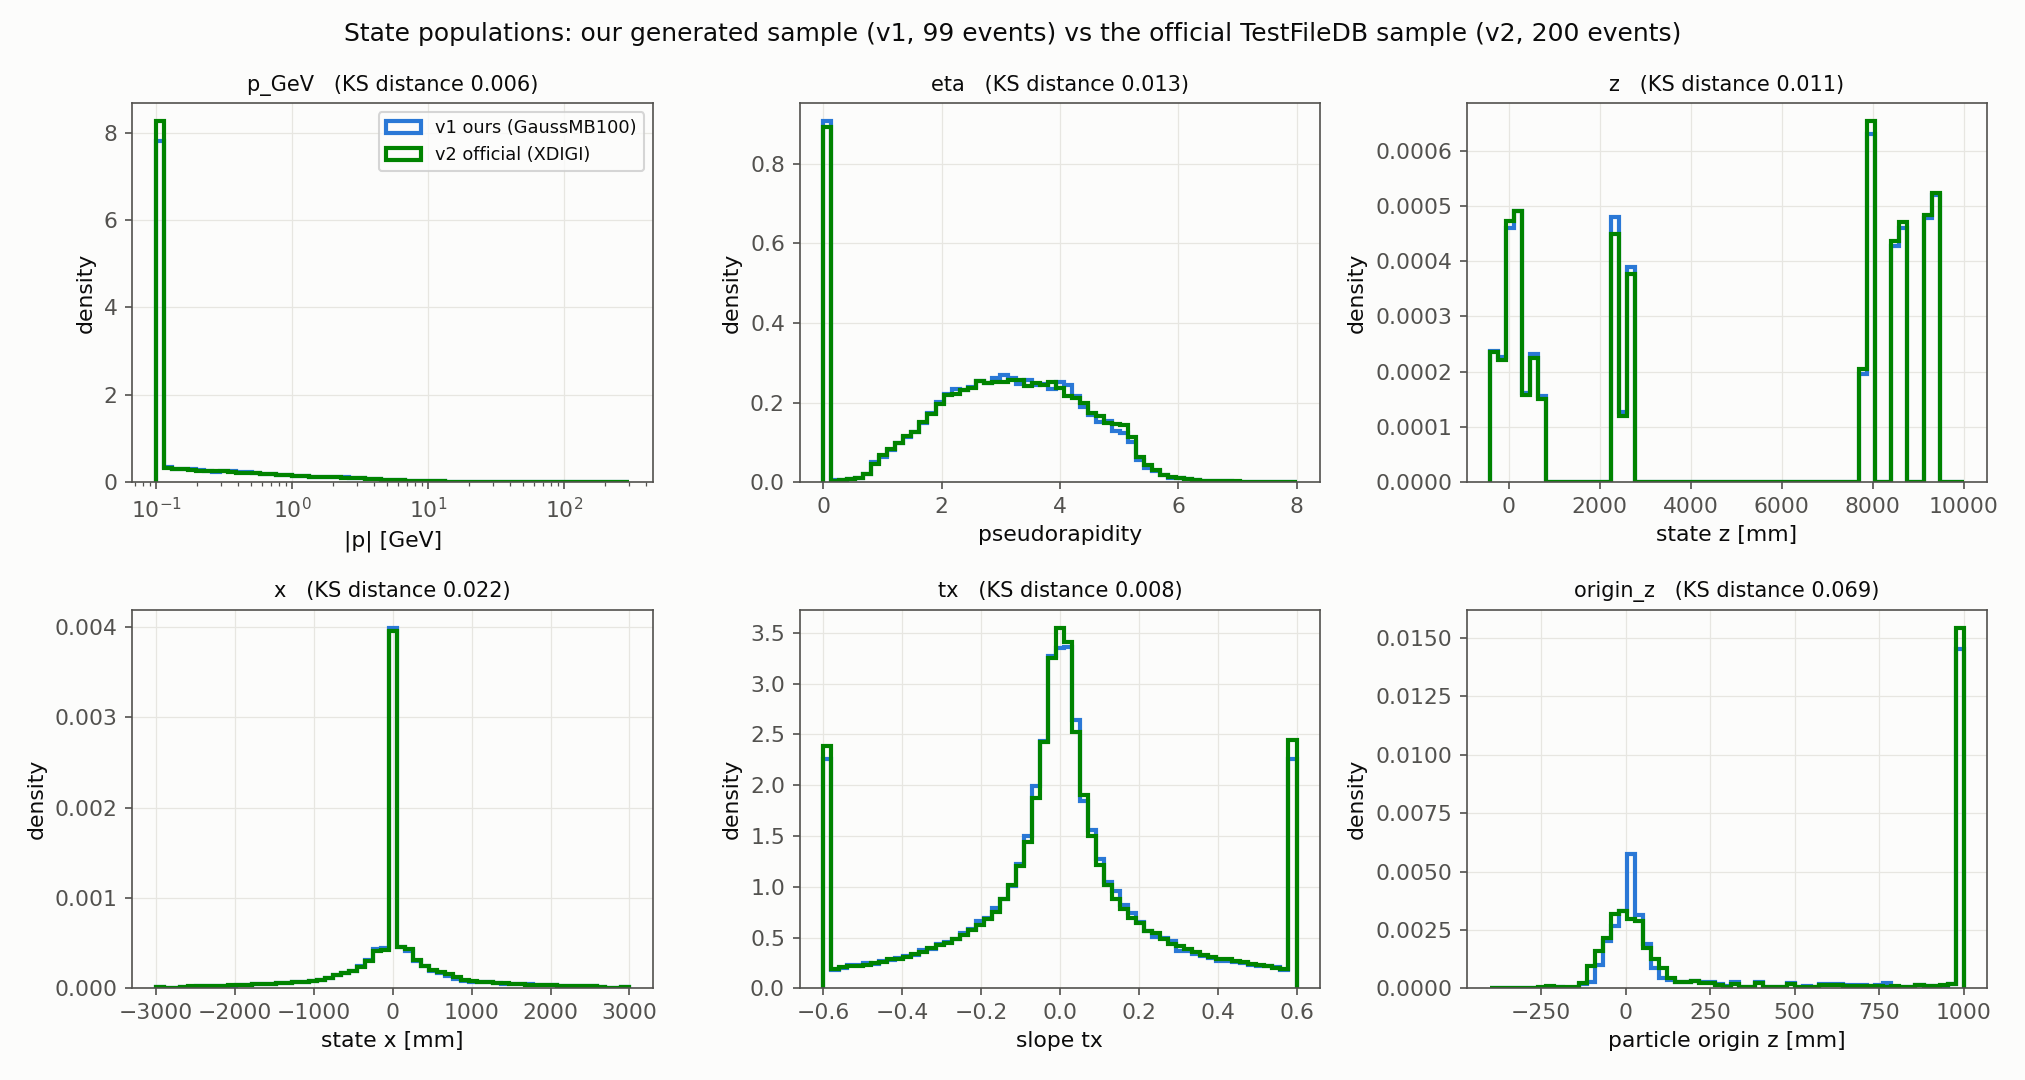
\includegraphics[width=0.92\linewidth]{fig_population.png}
  \caption{The population the surrogate is trained on, compared between the
  sample generated in-house in July (v1, $99$ events) and the official
  TestFileDB sample that replaced it (v2, $200$ events). The six panels show
  momentum, pseudorapidity, the $z$ position of the harvested states, the
  transverse position $x$, the slope $t_x$, and the $z$ of the particle's
  production point, each as a normalised density with the Kolmogorov--Smirnov
  distance between the two samples printed in the panel title. The distributions
  agree closely, with distances $0.006$ to $0.069$, which is the check that
  switching to the official sample changed the provenance of the population and
  not its physics. The structure in the $z$ panel is the detector itself: the
  three clusters are the vertex detector around $z = 0$, the upstream tracker
  near $2400\mm$, and the scintillating-fibre tracker beyond $7800\mm$. The peak
  at $1000\mm$ in the origin panel is particles produced in material rather than
  at the collision point; those are kept in the sample and flagged, not hidden.}
  \label{fig:population}
\end{figure}

\subsection{The shared package and its three gates}

All experiment folders import one package,
\texttt{R/\_shared}, so that a difference between two
experiments is a difference in the experiment and never a drifted copy of the
physics or the optimiser. The package contains the field-map loader, the tableau
construction, the reference integrator, the differentiable field, the network,
the losses, the dataset builders, the scorers and the training driver. Three
gates protect it, and all three pass.

\begin{enumerate}
  \item \textbf{Vendoring parity.} The field-map loader was copied into this
  repository from its original location, and the copy is required to return
  bit-identical values to the original on $200{,}000$ random points inside the
  map. Measured difference: exactly $0.0$ tesla, and the map file's md5 matches.
  \item \textbf{Differentiable-field parity.} The physics loss needs the field
  as a function it can differentiate through, so there is a second
  implementation in PyTorch. It is required to agree with the numerical original
  to $10^{-12}$ T. Measured: $1.3 \times 10^{-15}$ T on both polarities.
  \item \textbf{Baseline reproduction.} The generalised code, with its
  generalisations switched off, must reproduce the verified July baseline bit
  for bit: the same dataset of $1979/2062/2018$ states with identical arrays,
  the same initial parameters, the same losses and gradients, and the first
  optimiser restart landing on the same number to the last bit.
\end{enumerate}

\subsection{Compute, and the single-thread caveat}

All training ran on the Nikhef HTCondor farm, one job per combination of
architecture, mode and seed, single-threaded and in double precision.
Multithreaded PyTorch spin-waits on these nodes and is about $68$ times slower,
so every job sets one thread before importing the library. A consequence worth
stating plainly is that runs from the September campaign are not bit-comparable
with the July runs, which used four threads: a different reduction order changes
the last bits, and $200$ line-searched iterations amplify that into the fourth
significant digit. Comparisons across that boundary are made at the level of
seed ranges, never digit for digit.

% ===========================================================================
\section{Results}
\label{sec:results}

This section reports the July baseline the campaign starts from, then each
experiment in turn, then assembles the verdict.

\subsection{The July baseline}
\label{sec:baseline}

By the end of July three things were fixed and have not been revisited since.

\textbf{The leg.} The experiments needed one concrete extrapolation step to work
on. I took the modal plane pair of the $11{,}046$ forward cross-magnet legs in
the training set: $z_0 = 2648.2\mm$, the last plane of the upstream tracker, to
$z_1 = 7826.0\mm$, the first plane of the scintillating-fibre tracker. The step
is $\Delta z = 5177.8\mm$ and it crosses the whole magnet. I call it the frozen
leg. It is the hardest of the routine steps and the one where a surrogate would
be most valuable.

\textbf{The number of stages, $q = 8$.} Chosen from the exact-scheme measurement
of Section~\ref{sec:floor}: at $q = 8$ the scheme's own error on this leg has
fallen to the field map's floor, and going further buys nothing.
Section~\ref{sec:stages} tests that choice properly.

\textbf{The first converged label-free result.} On the official sample, with the
fiducial requirement in place and trained to a confirmed stall, a network of
four layers of $50$ units with $q = 8$ reached the numbers of
Table~\ref{tab:baseline}.

\begin{table}[tbp]
  \centering
  \caption{The July baseline on the frozen cross-magnet leg, $4 \times 50$
  network, $q = 8$, three seeds. Test-split median endpoint error in
  micrometres, with the individual seeds in brackets. The two losses are
  indistinguishable within the seed spread. Source:
  \texttt{One\_step\_network\_v2/results/summary.csv}.}
  \label{tab:baseline}
  \small
  \begin{tabular}{lr}
    \toprule
    & endpoint error, $\um$ \\
    \midrule
    exact scheme, $q = 8$ (the ceiling) & $23$ \\
    network, label-free physics loss & $183$ \ [$177$, $183$, $235$] \\
    network, supervised data twin & $192$ \ [$162$, $192$, $208$] \\
    straight line (ignore the magnet) & $520{,}444$ \\
    \bottomrule
  \end{tabular}
\end{table}

\begin{figure}[tbp]
  \centering
  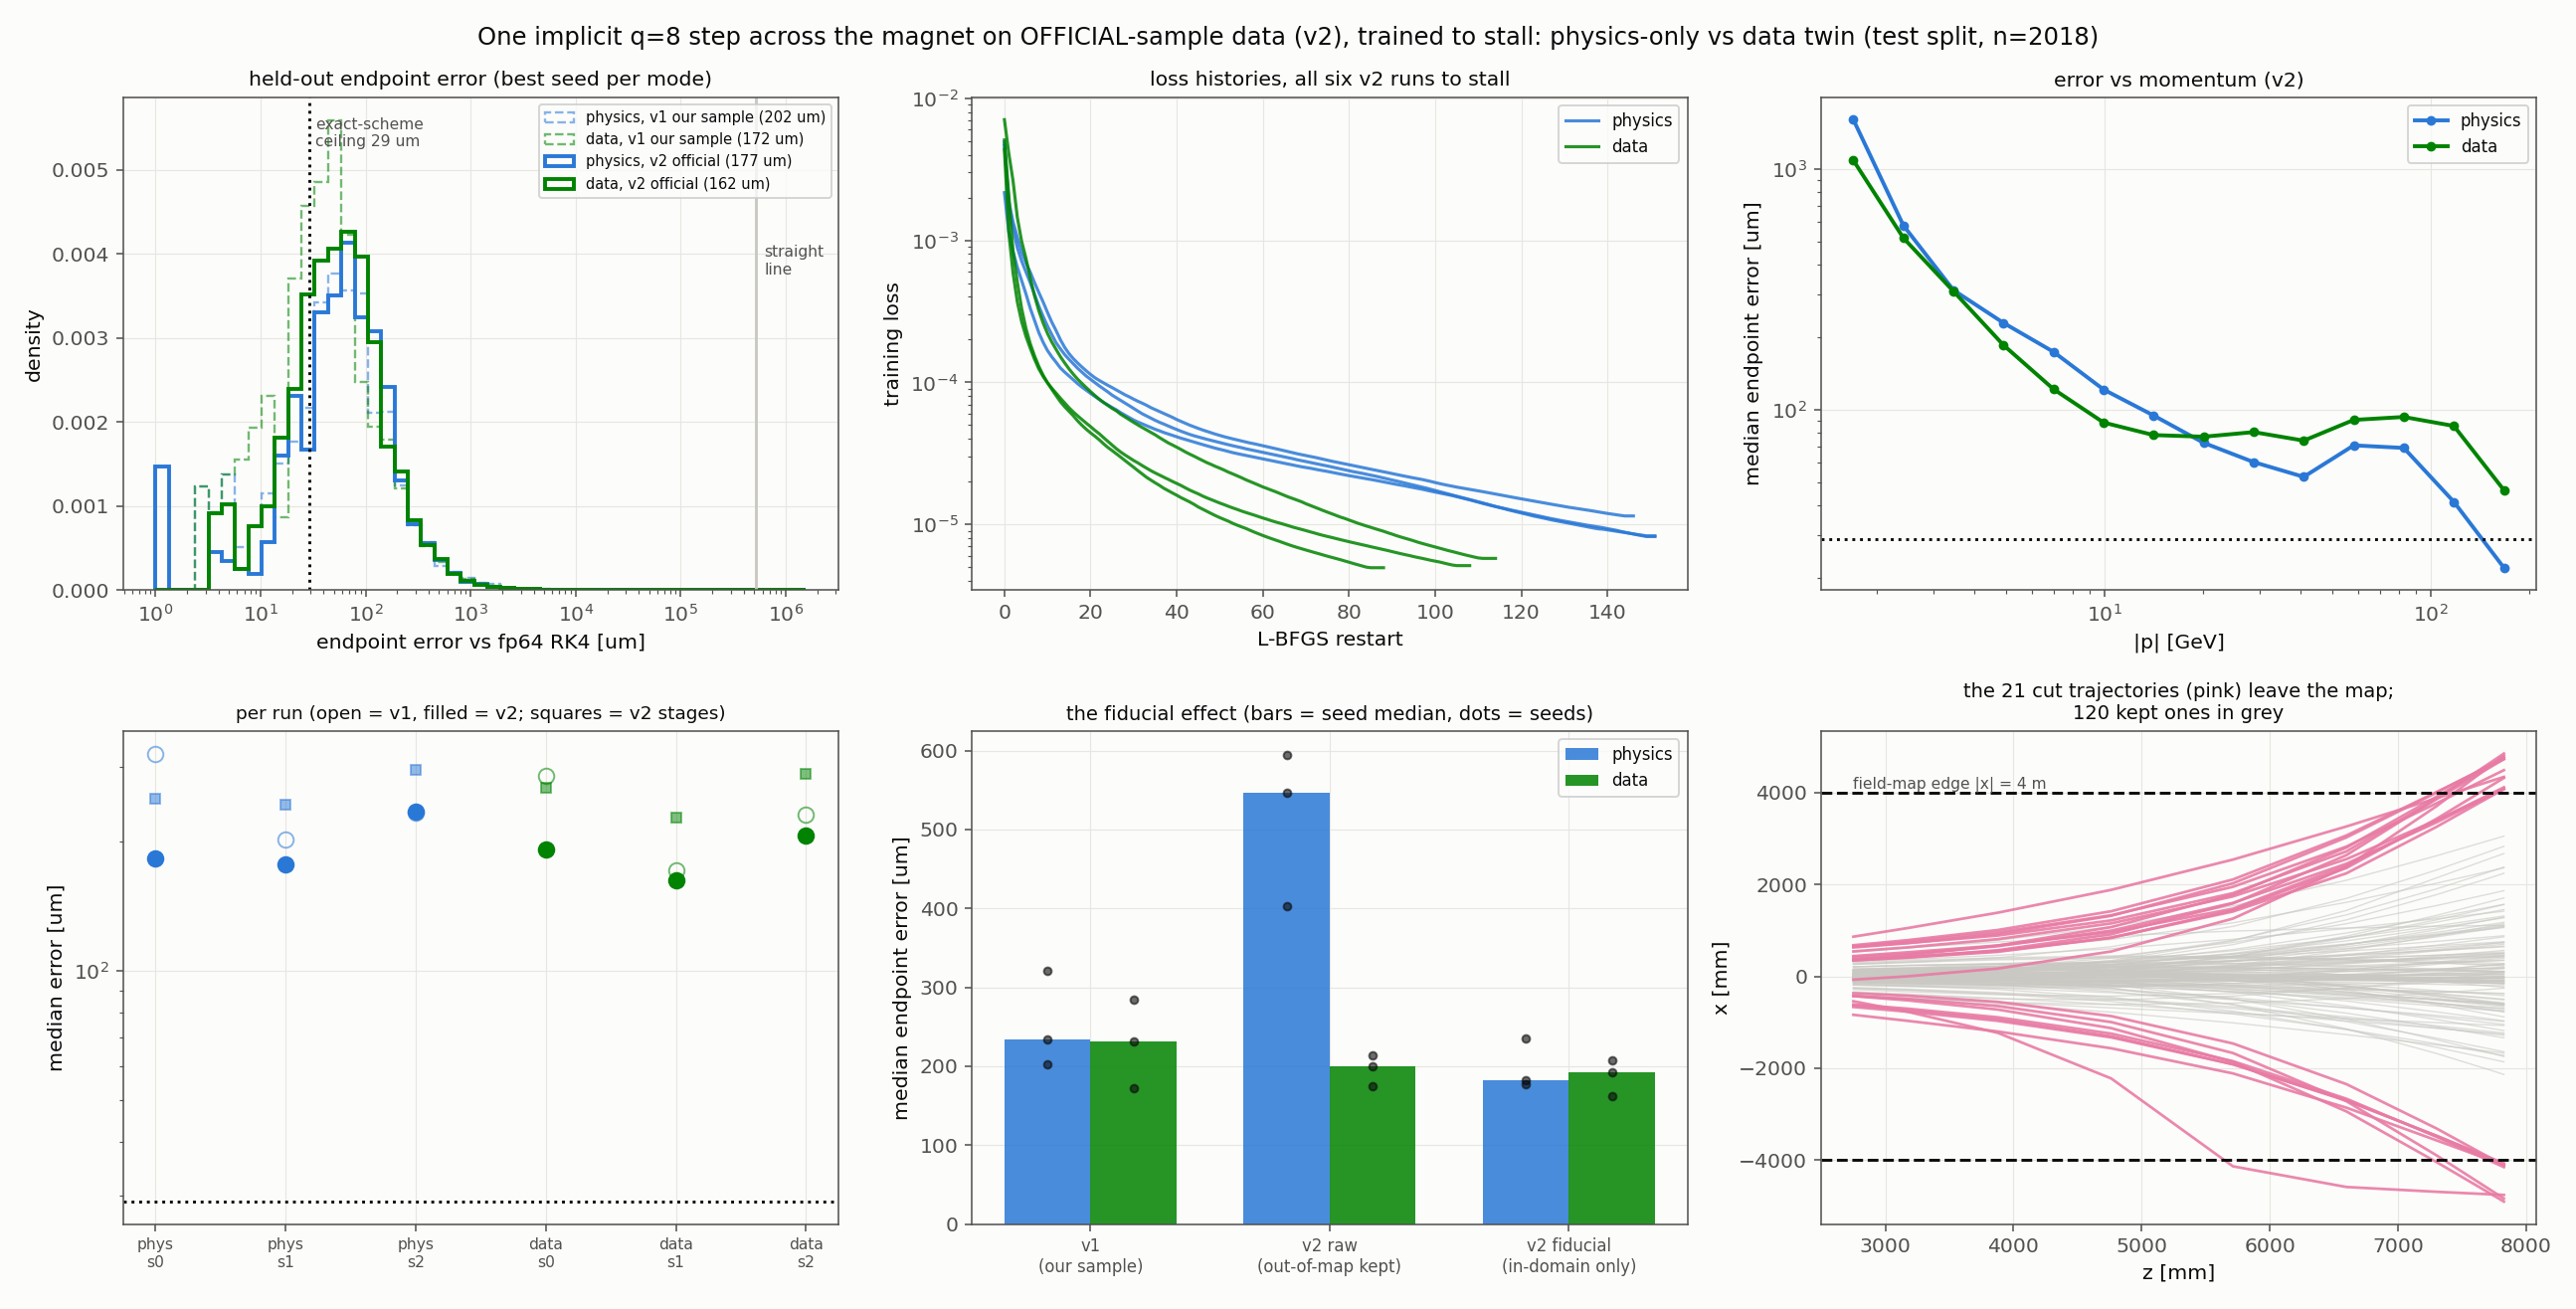
\includegraphics[width=0.86\linewidth]{fig_baseline.png}
  \caption{The July baseline on the frozen magnet crossing. The panels show the
  distribution of test-split endpoint errors for the three label-free seeds and
  the three supervised seeds, the training histories per optimiser restart with
  the confirmation pass marked, and the comparison against the in-house sample
  the official one replaced. The point of the figure is the overlap of the two
  loss families: with the fiducial requirement of Section~\ref{sec:fiducial} in
  place, the label-free loss and the supervised twin are not distinguishable at
  three seeds on this leg.}
  \label{fig:baseline}
\end{figure}

That is the result the September campaign set out to interrogate.

\subsection{How many stages the magnet crossing needs}
\label{sec:stages}

\textbf{Question.} Is $q = 8$ the right working point, and in the regimes where
the scheme itself is inaccurate, does the label-free network reproduce the
scheme's own error?

\textbf{Design.} Vary $q$ over $\{2, 4, 8, 16\}$ and nothing else: same
population, same fiducial cut, same $4 \times 50$ network, same protocol, same
split seed. Both losses, three seeds each, $24$ runs. For each $q$ the exact
scheme is also solved by root-finder on the very same $2018$ test states, so the
ceiling is like for like.

\begin{table}[tbp]
  \centering
  \caption{Stage-count sweep on the frozen cross-magnet leg. Test-split median
  endpoint error in micrometres, median over three seeds with the seed range in
  brackets. The ceiling is the same $q$-stage scheme solved directly by a
  root-finder on these same $2018$ test states. The straight line is
  $520{,}444\um$ at every $q$. All $24$ runs converged. Source:
  \texttt{Stage\_count\_sweep/results/error\_vs\_stages.csv}.}
  \label{tab:stages}
  \small
  \begin{tabular}{ccccc}
    \toprule
    stages $q$ & physics loss & data twin & exact scheme & exact scheme, p95 \\
    \midrule
    $2$  & $5202$ [$5199$--$5218$] & $174$ [$168$--$223$] & $5198$ & $37{,}728$ \\
    $4$  & $5371$ [$5352$--$5394$] & $181$ [$157$--$181$] & $5401$ & $54{,}057$ \\
    $8$  & $181$ [$165$--$240$]    & $176$ [$162$--$204$] & $23$   & $1610$ \\
    $16$ & $187$ [$186$--$280$]    & $170$ [$147$--$176$] & $20$   & $325$ \\
    \bottomrule
  \end{tabular}
\end{table}

The first two rows are the most informative result in the campaign. At $q = 2$
the label-free network lands at $5202\um$ against a ceiling of $5198\um$, within
$0.1$ percent. At $q = 4$ it lands at $5371\um$ against $5401\um$, within $0.6$
percent. The network is not failing. It is solving the equations it was given,
and those equations are $5\mm$ wrong on this leg. This is the cleanest available
demonstration that the physics loss of Eq.~\eqref{eq:loss} does what it claims:
it drives the network onto the solution of the discrete scheme, whatever that
solution happens to be. The supervised twin at the same $q$ sits at $174$ and
$181\um$, thirty times better, because its labels are the true trajectory and it
never sees the scheme at all.

Between $q = 4$ and $q = 8$ the ceiling falls from $5401\um$ to $23\um$ and
crosses below the network's own floor. From there the limiting factor is the
network and the optimiser rather than the discretisation, and $q = 16$ agrees
with $q = 8$ within the seed spread, $187$ against $181\um$, while costing $68$
outputs per sample instead of $36$. That fixes $q = 8$ as the working point.

Two things were not expected. First, $q = 4$ is no better than $q = 2$ and is
slightly worse at the ceiling, $5401$ against $5198\um$. Formal order $2q$ is an
asymptotic statement about small steps, and a single $5178\mm$ step through a
magnet is nowhere near that regime; the extra stages buy nothing until there are
enough of them to resolve the field variation along the leg, and between four
and eight there suddenly are. The root-finder converged to a residual below
$10^{-8}$ on $99.9$ percent of legs at every $q$, so these are genuine solutions
of the discrete equations. The equations are simply far from the differential
equation. Second, $q = 16$ is not the hard case: it trains faster than $q = 8$,
$113$ to $115$ restarts against $154$. The hardest optimisation in the grid is
$q = 4$.

\paragraph{The \texorpdfstring{$29\um$}{29 micrometre} correction.}
A ceiling must always be quoted on the population being scored. An earlier
measurement of the exact scheme, made on $32$ legs drawn stratified in momentum
and each on its own start plane, gave $29\um$ at $q = 8$, and that number was
quoted in July. Stratifying in momentum deliberately over-weights the soft,
hard-bending tracks, so the stratified figure describes a harder population than
any test split used here. On the $2018$ frozen-leg test states with their natural
momentum mix the ceiling is $23\um$, and the pre-stated ceilings of about
$14\mm$ at $q = 2$ and $4.3\mm$ at $q = 4$ become $5198$ and $5401\um$. Both
curves are carried in Figure~\ref{fig:stages} so that the difference is visible
rather than argued about. The qualitative claim survives intact: the physics
network tracks the ceiling at low $q$ and leaves it at $q = 8$.

\begin{figure}[tbp]
  \centering
  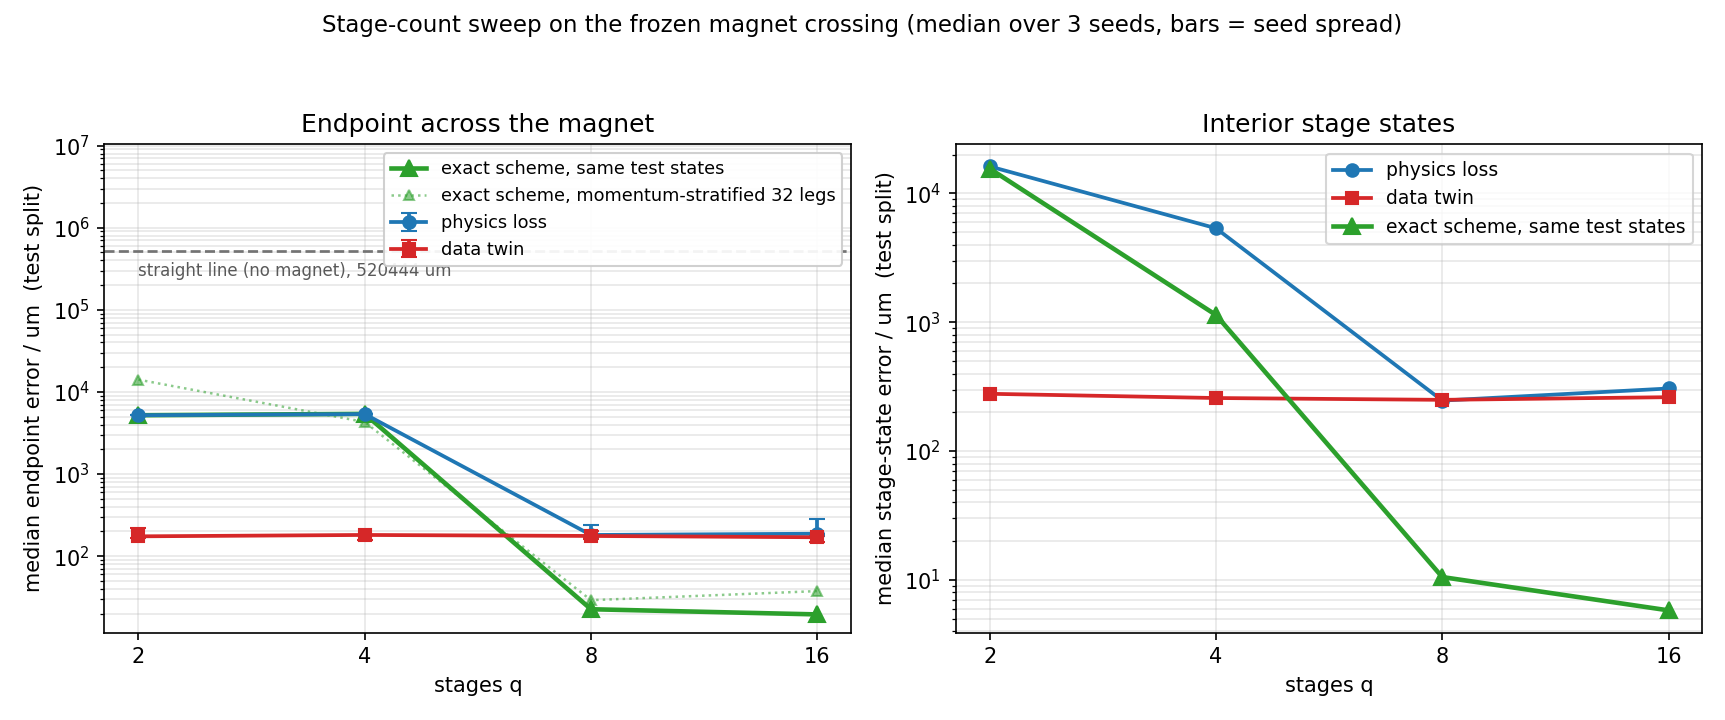
\includegraphics[width=0.88\linewidth]{fig_stages.png}
  \caption{Median test-split endpoint error against the number of
  Gauss--Legendre stages $q$, on a logarithmic vertical axis, for the frozen
  cross-magnet leg. The left panel is the endpoint of the step; the right panel
  is the same measure taken over the eight interior stage states. Blue is the
  label-free physics loss, red the supervised twin, solid green the exact scheme
  solved by root-finder on the very same test states, and dotted green the same
  scheme measured on the momentum-stratified sample of $32$ legs, which
  over-weights the hardest tracks and gives a different and non-comparable
  number. Bars are the spread over three seeds. The dashed horizontal line at
  $520{,}444\um$ is the straight-line baseline. The blue and green curves lie on
  top of one another at $q = 2$ and $q = 4$, which is the physics loss
  reproducing the scheme's own error; they separate at $q = 8$, where the
  scheme's error drops below the network's floor and the network becomes the
  limiting factor. The red curve is flat at about $175\um$ at every $q$, because
  the supervised twin never sees the scheme.}
  \label{fig:stages}
\end{figure}

\subsection{Network size, seeds, and what sets the floor}
\label{sec:size}

\textbf{Question.} The frozen-leg network stops at about $180$ to $220\um$ while
the scheme it is solving reaches $23\um$. Is the gap a limit of the network's
representational capacity, or of the optimiser's ability to find the good
weights? And which network should the later experiments use?

\textbf{Design.} The July experiment with two things varied: width in
$\{32, 50, 100, 200\}$ crossed with depth in $\{2, 4, 6\}$, and seeds $0$ to
$9$. That is $120$ label-free runs, plus $10$ supervised runs at the winning
architecture, so $130$ runs.

\begin{table}[tbp]
  \centering
  \caption{Architecture grid on the frozen cross-magnet leg at $q = 8$, ordered
  by parameter count. Test-split median endpoint error in micrometres over the
  converged seeds, with the best and worst converged seed. Unconverged runs are
  never pooled into a median. The last row is the supervised twin at the winning
  architecture. Source:
  \texttt{Network\_size\_and\_seed\_study/results/by\_architecture.csv}.}
  \label{tab:grid}
  \small
  \begin{tabular}{llrcrrrl}
    \toprule
    loss & depth $\times$ width & parameters & converged & median & min & max
      & median final loss \\
    \midrule
    physics & $2 \times 32$  & $2{,}436$   & $5/10$  & $1059$ & $853$ & $1600$ & $1.83\times10^{-4}$ \\
    physics & $2 \times 50$  & $4{,}686$   & $9/10$  & $470$  & $340$ & $593$  & $4.54\times10^{-5}$ \\
    physics & $4 \times 32$  & $4{,}548$   & $3/10$  & $411$  & $387$ & $450$  & $5.37\times10^{-5}$ \\
    physics & $6 \times 32$  & $6{,}660$   & $4/10$  & $427$  & $391$ & $2725$ & $6.51\times10^{-5}$ \\
    physics & $4 \times 50$  & $9{,}786$   & $10/10$ & $222$  & $165$ & $244$  & $1.06\times10^{-5}$ \\
    physics & $2 \times 100$ & $14{,}336$  & $10/10$ & $223$  & $201$ & $299$  & $1.08\times10^{-5}$ \\
    physics & $6 \times 50$  & $14{,}886$  & $6/10$  & $326$  & $248$ & $525$  & $2.74\times10^{-5}$ \\
    physics & $4 \times 100$ & $34{,}536$  & $10/10$ & $133$  & $128$ & $156$  & $3.04\times10^{-6}$ \\
    physics & $2 \times 200$ & $48{,}636$  & $10/10$ & $153$  & $128$ & $241$  & $4.19\times10^{-6}$ \\
    physics & $6 \times 100$ & $54{,}736$  & $10/10$ & $191$  & $152$ & $242$  & $9.33\times10^{-6}$ \\
    physics & $4 \times 200$ & $129{,}036$ & $10/10$ & $115$  & $100$ & $134$  & $2.06\times10^{-6}$ \\
    physics & $6 \times 200$ & $209{,}436$ & $9/10$  & $159$  & $150$ & $208$  & $6.05\times10^{-6}$ \\
    \midrule
    data twin & $4 \times 200$ & $129{,}036$ & $10/10$ & $128$ & $105$ & $159$ & $1.34\times10^{-6}$ \\
    \bottomrule
  \end{tabular}
\end{table}

Four things follow from Table~\ref{tab:grid}.

\textbf{The floor is set by the optimiser, not by capacity.} Growing the network
from $2436$ to $129{,}036$ parameters, a factor $53$, moves the median from
$1059\um$ to $115\um$, a factor $9.2$, and the returns collapse along the way:
the last width doubling, $4 \times 100$ to $4 \times 200$, buys $14$ percent for
$3.7$ times the parameters and $1.8$ times the wall time. The decisive evidence
is the correlation. Over all $96$ converged label-free runs the Spearman rank
correlation between the final training loss and the test endpoint error is
$+0.965$. Every architecture and every seed lies on one band, three decades of
loss mapping monotonically onto one and a half decades of error. The endpoint
error is a readout of how far the optimiser got, not of what the network could
represent. A wider network helps only because L-BFGS gets further down on it:
the $4 \times 50$ networks stall at a median final loss of
$1.06 \times 10^{-5}$, the $4 \times 200$ networks at $2.06 \times 10^{-6}$. It
follows that anything improving the conditioning of the optimisation problem
should be expected to pay more than more parameters do, which is the prediction
Section~\ref{sec:residual} tests.\footnote{This is the same number, to the
second decimal place, that the van der Pol study measured on a two-dimensional
autonomous oscillator with an analytic right-hand side. I did not expect two
systems with that little in common to agree that closely, and I have no
explanation for it beyond the shared optimiser.}

\textbf{Depth 4 is the optimum, and it is interior.} Depth $6$ is never better
than depth $4$ and is $39$ to $47$ percent worse at widths $50$, $100$ and
$200$; it is also much harder to train, with $4$, $6$, $10$ and $9$ seeds of ten
converging at the four widths against $3$, $10$, $10$ and $10$ at depth $4$.
Depth $2$ is worse than depth $4$ at every width, by $33$ percent at width $200$
rising to $158$ percent at width $32$.

\textbf{At the largest size the label-free loss beats its own supervised twin.}
At $4 \times 200$ the physics loss gives $115\um$ [$100$--$134$] against the
twin's $128\um$ [$105$--$159$], so the twin's median is $12$ percent higher. The
twin also has the wider seed spread, a factor $1.51$ between its best and worst
seed against $1.33$, while reaching its stall in about half the restarts. The
factor-two gap that the July experiments chased is gone. With the fiducial
requirement in place and a network large enough for the optimiser to work with,
a loss that never sees a label matches and slightly beats supervision on labels
computed with the same field.

\textbf{Seeds must be pooled, and validation selection is safe for the one-step
task.} Over architectures with at least three converged seeds, the median ratio
between the luckiest and unluckiest seed is $1.54$. It shrinks with size, to
$1.22$ at $4 \times 100$ and $1.33$ at $4 \times 200$. Choosing a seed on
validation endpoint error is reliable here: the rank correlation between
validation and test endpoint error over the $96$ converged runs is $+0.995$, the
validation-best seed is also the test-best seed in $9$ of $12$ architectures,
and where it is not, the penalty is at most $2.3$ percent.
Section~\ref{sec:general} shows that this stops being true the moment the
network is chained.

The recommendation this experiment produced, and which the general-leg
experiment then only partly followed because it was already running, was
$4 \times 100$ as the smallest adequate network, with $4 \times 200$ as the
check that a result is not size-limited. $4 \times 50$ sits on the steep part of
the curve, where a result reports the network size as much as the physics.

\begin{figure}[tbp]
  \centering
  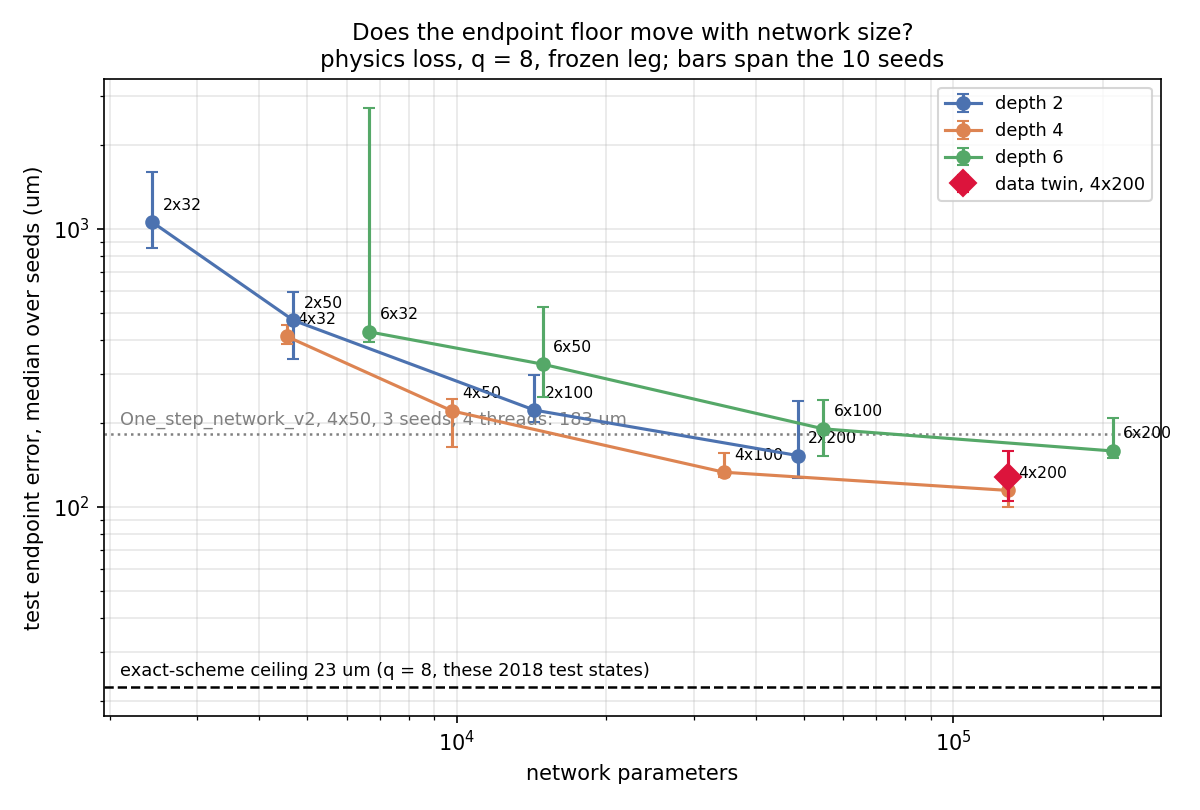
\includegraphics[width=0.62\linewidth]{fig_architecture.png}
  \caption{Median test endpoint error against the number of network parameters,
  both axes logarithmic, for the label-free loss on the frozen magnet crossing
  at $q = 8$. Each point is one architecture, labelled depth $\times$ width; the
  three coloured curves are depths $2$, $4$ and $6$, and the bars span the ten
  seeds. The red diamond is the supervised twin at $4 \times 200$. The dotted
  horizontal line marks the July three-seed baseline at $183\um$ and the dashed
  line at the bottom marks the exact-scheme ceiling of $23\um$ on these same
  $2018$ test states. Depth $4$ lies below depths $2$ and $6$ at every width,
  and the depth-$4$ curve flattens above about thirty thousand parameters, so
  that the last factor $3.7$ in size buys $14$ percent in error. The gap between
  the flattening curve and the ceiling is the factor $5$ that this study
  attributes to the optimiser rather than to capacity.}
  \label{fig:architecture}
\end{figure}

\begin{figure}[tbp]
  \centering
  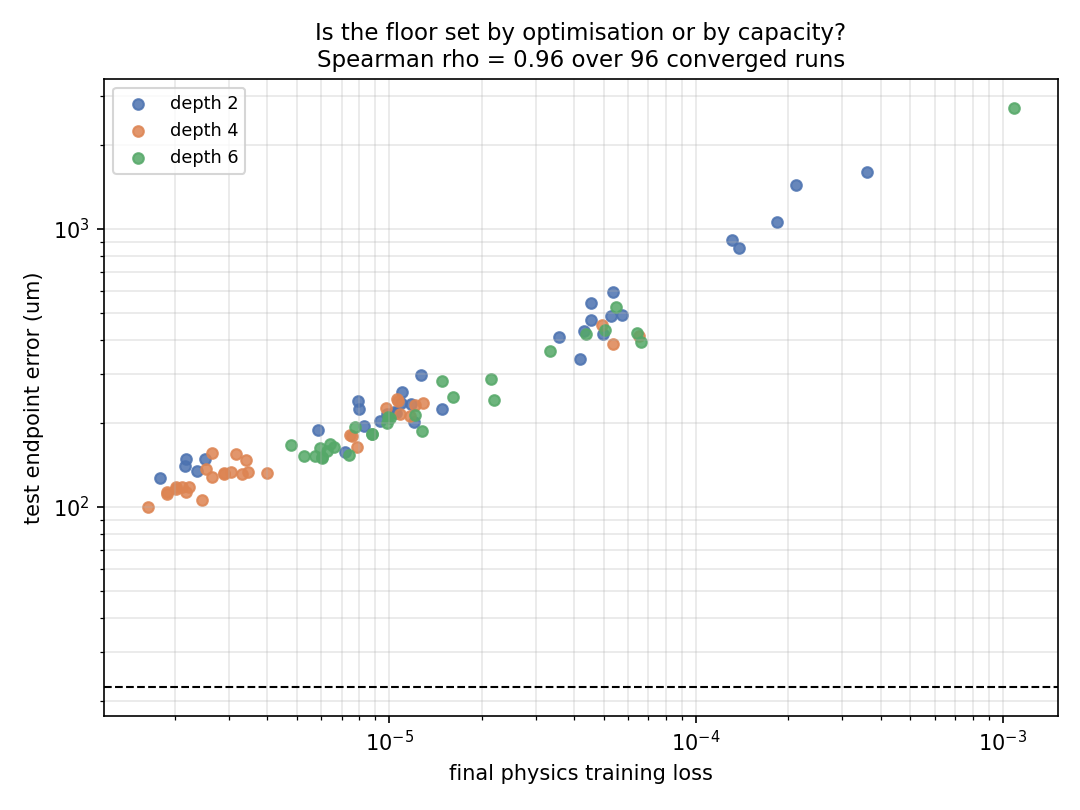
\includegraphics[width=0.52\linewidth]{fig_loss_vs_error.png}
  \caption{The evidence behind the optimisation-floor claim: final training loss
  against test-split endpoint error, both axes logarithmic, one point per
  converged label-free run, coloured by architecture. All $96$ converged runs
  lie on a single band, three decades of loss mapping monotonically onto one and
  a half decades of error, with a Spearman rank correlation of $+0.965$. If the
  floor were a capacity limit the small architectures would sit above the band
  at their own loss values, forming separate branches. They do not.}
  \label{fig:lossvserror}
\end{figure}

\subsection{Training where no labels exist: the reversed magnet polarity}
\label{sec:magnetup}

\textbf{Question.} The claim of the technique is that no labels are needed. The
strongest available test of that claim is to train on a configuration for which
no labelled sample has ever been produced. LHCb periodically reverses the
magnet's polarity, so there is a second field map, and no training labels have
ever been made for it in this project.

\textbf{Design.} The identical $4 \times 50$ network, the identical protocol,
the identical training population, with the single change that the loss is built
on the reversed map. Label-free seeds $0$ to $9$ plus three supervised control
runs, so $13$ runs, all converged. The reversed-polarity references exist only
to score; the label-free runs never see them.

Three checks were run before submitting. The two maps are exactly one another's
negative: on $200{,}000$ random in-map points the maximum of
$|\mathbf{B}_{\mathrm{up}} + \mathbf{B}_{\mathrm{down}}|$ is $0.0$ in all three
components, so the field magnitude profile is bit-for-bit identical and only the
sign of the bending differs. Both polarities are built from the same event rows,
since the selection uses no field at all. And a probe run established that the
polarity flag really reaches the loss and is not silently ignored: one optimiser
restart from the same seed on the same states gives $2.62 \times 10^{-3}$ with
the loss built on the reversed map against $8.03 \times 10^{-3}$ with it built
on the original.

\begin{table}[tbp]
  \centering
  \caption{The reversed magnet polarity against the original, on the frozen
  cross-magnet leg, $4 \times 50$, $q = 8$. Test-split median endpoint error in
  micrometres, median over seeds with the seed range in brackets. No labelled
  sample has ever been produced for the reversed polarity in this project.
  Source: \texttt{Magnet\_up\_field/results/summary.csv} and
  \texttt{Magnet\_up\_field/results/ceiling\_summary.json}.}
  \label{tab:magnetup}
  \small
  \begin{tabular}{lrr}
    \toprule
    quantity & magnet up & magnet down \\
    \midrule
    network, label-free physics loss & $229$ [$171$--$296$], 10 seeds
                                     & $222$ [$165$--$244$], 10 seeds \\
    network, supervised data twin    & $204$ [$187$--$230$], 3 seeds
                                     & $192$ [$162$--$208$], 3 seeds \\
    exact-scheme ceiling on the test states & $22.1$ & $22.5$ \\
    straight line & $525{,}184$ & $520{,}444$ \\
    network divided by its own ceiling & $10.4\times$ [$7.7$--$13.4$]
                                       & $9.8\times$ [$7.2$--$10.8$] \\
    \bottomrule
  \end{tabular}
\end{table}

The label-free network reaches the same floor on the reversed field as on the
original and sits the same distance above the reversed field's own ceiling. The
two ten-seed ranges overlap almost completely, and the four percent difference
in medians is far inside a seed spread that is itself a factor $1.7$ wide on the
reversed polarity and $1.5$ on the original. It also matches its own supervised
twin on both, $229$ against $204\um$ and $222$ against $192\um$. Both are three
orders of magnitude below the straight line, so the network has learned the
bending and not merely the geometry, and it has learned it with the correct
sign.

One genuine asymmetry was found, and it is in the tracks rather than in the map.
The fiducial requirement removes $21$, $20$ and $15$ states from the three
splits on the original polarity and \emph{none} on the reversed one: the
sample's charge and angular distribution is not symmetric in $x$, and the
original polarity is the one that bends these particular soft tracks out of the
map while the reversed polarity bends them back in. The same asymmetry appears
in the exact scheme's worst case, $38\mm$ reversed against $258\mm$ original. A
control that re-scores the reversed networks on only the $2018$ tracks the
original polarity also keeps moves the median from $229.4$ to $226.6\um$, about
one percent, so the medians are unaffected. Statements about tails, however,
must say which polarity they refer to.

\begin{figure}[tbp]
  \centering
  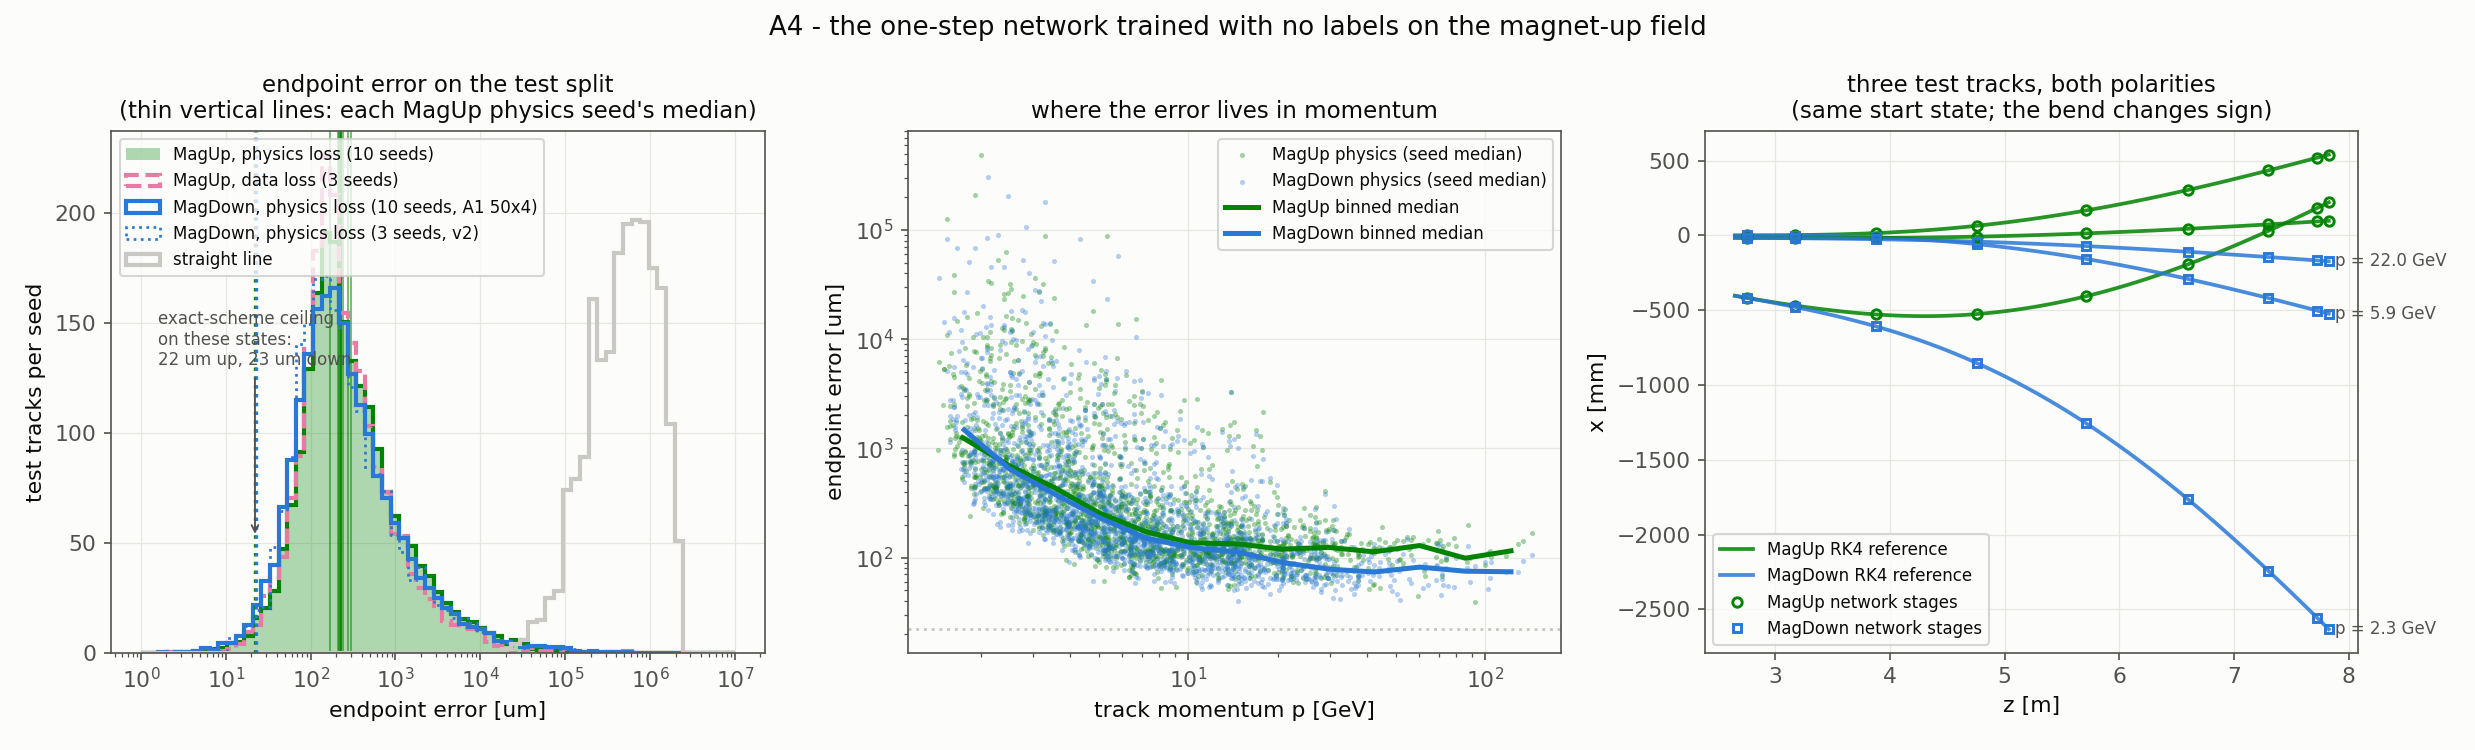
\includegraphics[width=\linewidth]{fig_magnet_up.png}
  \caption{Three panels summarising the reversed-polarity experiment. Left: the
  distribution of test-split endpoint errors on a logarithmic horizontal axis,
  with the ten reversed-polarity label-free seeds in filled green, the three
  reversed-polarity supervised seeds in dashed pink, the ten original-polarity
  label-free seeds in solid blue, the three July original-polarity seeds in
  dotted blue, and the straight-line baseline in grey near one million
  micrometres; the two polarities lie on top of one another and the two
  exact-scheme ceilings, $22$ and $23\um$, are marked at the left. Middle:
  endpoint error against track momentum with binned medians overlaid; the two
  polarities trace the same curve, falling from about one millimetre at $2$ GeV
  to about $100\um$ above $20$ GeV. Right: three test tracks propagated from the
  same start states under both polarities, with the network's eight stage states
  as markers on the reference curves; the trajectories curve in opposite
  directions, which is the check that the network learned the sign of the
  bending and not merely the geometry.}
  \label{fig:magnetup}
\end{figure}

\subsection{One network for every kind of step, with absolute outputs}
\label{sec:general}

\textbf{Question.} Everything so far trains a network on one frozen leg: every
sample starts on the same plane and ends on the same plane, so the network
cannot be used anywhere else. Two things have to be true before this is a usable
extrapolator. One network must serve steps of arbitrary length starting
anywhere, and it must survive being applied repeatedly to its own output.

\textbf{Design.} The leg becomes an input. Each sample carries its own start
plane $z_0$ and its own step length $\Delta z$, normalised and handed to the
network as two extra inputs, and the stage planes become per-sample quantities
$z_0 + c_j \Delta z$ rather than constants. One network is asked to serve leg
types A, B and C at once. The training size was fixed by a rule stated before
any result was looked at, namely the largest of $2000$, $4000$, $8000$ and
$16000$ for which one optimiser restart runs in under $90$ seconds, giving
$N = 8000$, or $7935$ train, $3969$ validation and $3961$ test states after the
fiducial cut. The leg mix is the training set's own and is not stratified:
$1317$ of type A, $1060$ of type B and $5558$ of type C in the train split.
Architectures $4 \times 50$ and $4 \times 100$, label-free seeds $0$ to $9$,
supervised seeds $0$ to $2$, so $26$ runs, all converged. A second wave at
$4 \times 200$ followed overnight, $13$ runs of which $12$ converged.

\begin{table}[tbp]
  \centering
  \caption{One network for legs A, B and C with absolute outputs. Test-split
  median endpoint error in micrometres, median over converged seeds, with the
  seed range in brackets where quoted. The ceiling is the exact $q = 8$ scheme
  solved on this experiment's own test states, which is why it differs from the
  stratified numbers of Section~\ref{sec:stages}. The $4 \times 200$ column
  excludes one unconverged physics seed. Source:
  \texttt{General\_leg\_network/results/by\_leg.csv}.}
  \label{tab:general}
  \footnotesize
  \setlength{\tabcolsep}{3pt}
  \begin{tabular}{lrrrrrrrr}
    \toprule
    & \multicolumn{3}{c}{physics loss} & \multicolumn{3}{c}{data twin}
    & & \\
    \cmidrule(lr){2-4}\cmidrule(lr){5-7}
    leg & $4\times50$ & $4\times100$ & $4\times200$
        & $4\times50$ & $4\times100$ & $4\times200$
        & straight & ceiling \\
    \midrule
    A vertex fetch, $341\mm$   & $849$  & $404$  & $229$  & $653$  & $385$ & $227$ & $10.9$     & $0.0013$ \\
    B cross-magnet, $5175\mm$  & $6742$ & $2600$ & $1740$ & $2395$ & $933$ & $777$ & $444{,}075$ & $46$ \\
    C plane-to-plane, $70\mm$  & $535$  & $300$  & $213$  & $486$  & $235$ & $182$ & $6.6$      & $6\times10^{-7}$ \\
    \bottomrule
  \end{tabular}
\end{table}

One label-free network does serve all three leg types, and it does so nowhere
near any of their ceilings. On the cross-magnet leg the best label-free network
at $4 \times 100$ sits at $2600\um$ against a $46\um$ ceiling, a factor $56$.
Compared with the frozen-leg network of Section~\ref{sec:baseline} on the same
kind of leg, $183\um$, making the leg an input costs a \textbf{factor 14}, and
it costs a factor $11.7$ against the ten-seed frozen-leg figure of $222\um$ even
though the general network is twice as wide. On the two short leg types the
network is worse than doing nothing: ignoring the magnet entirely gives
$10.9\um$ on leg A and $6.6\um$ on leg C, while the network gives $404\um$ and
$300\um$.

Width keeps paying on the one-step score, with clear diminishing returns. Leg B
goes $6742 \to 2600 \to 1740\um$ for widths $50 \to 100 \to 200$, factors of
$2.6$ then $1.5$ for each doubling, and is still $38$ times above the $46\um$
ceiling. On the short legs the widest network is still $32$ times (leg C) and
$21$ times (leg A) worse than ignoring the magnet entirely, which no amount of
width can fix.

The supervised twin is uniformly ahead here, by a factor $2.8$ on leg B at
$4 \times 100$ and by $5$ to $25$ percent on legs A and C, where on the frozen
leg the two were indistinguishable. The gap between the two losses opens exactly
where the leg geometry varies. Where the error sits inside the step is also
informative: on legs A and C it is flat across the eight Gauss nodes, which is
the signature of a scale error rather than an accumulation, while on leg B it
grows monotonically from the first node to the endpoint, roughly doubling, which
is the bend being under-resolved.

\begin{figure}[tbp]
  \centering
  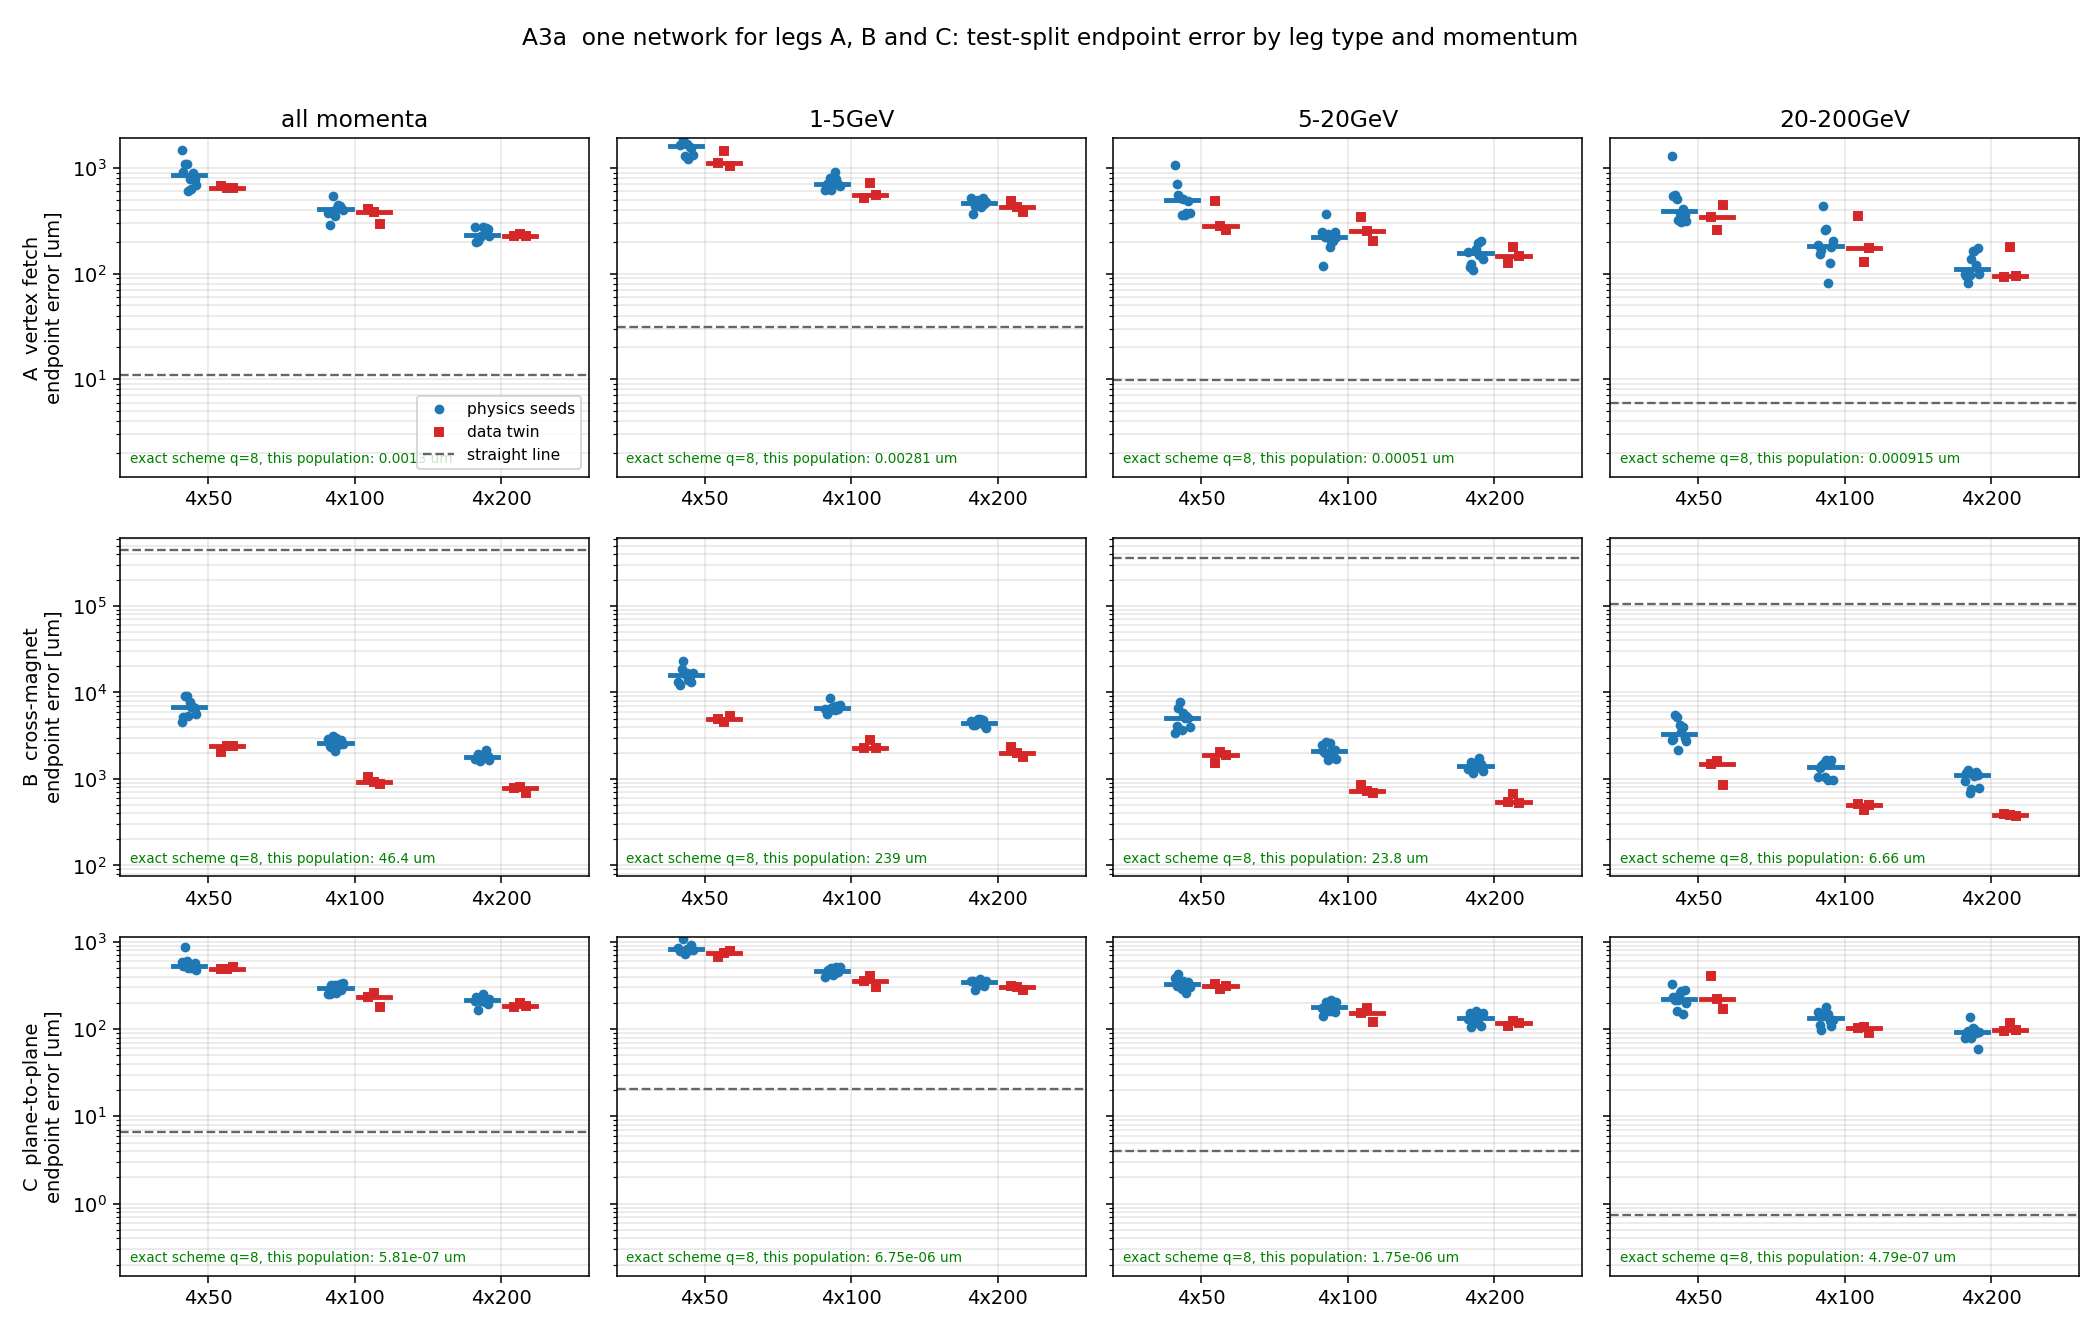
\includegraphics[width=0.78\linewidth]{fig_general_legs.png}
  \caption{Test-split endpoint error for the single general network with
  absolute outputs, by leg type (rows: A vertex fetch, B cross-magnet, C
  plane-to-plane) and momentum band (columns: all momenta, then $1$ to $5$, $5$
  to $20$ and $20$ to $200$ GeV), on a logarithmic vertical axis. Blue circles
  are the ten label-free seeds and red squares the three supervised seeds, with
  horizontal bars at the median; the dashed grey line in each panel is the
  straight-line baseline and the green annotation gives the exact-scheme ceiling
  on that same population. The middle row shows the network beating the straight
  line by two orders of magnitude on the cross-magnet leg while sitting a factor
  $56$ above the ceiling; the top and bottom rows show the opposite situation,
  where the straight line lies below every network point.}
  \label{fig:generallegs}
\end{figure}

\subsubsection{Chaining: the network walked along real particle paths}

For each test particle I collect the planes named by its stored forward legs,
sort them, and call consecutive planes a leg. The chain starts from the state at
the first plane, and the truth is the double-precision Runge--Kutta path from
that same start state through the same planes, so the network and the reference
begin in the same place and only the propagation is compared. Kept: $4563$ test
particles with four or more legs, $23{,}500$ legs in total, median leg length
$70\mm$ and 99th percentile $5.2$ m. All trained networks were walked along all
of them.

The obvious rule, that row $i$ is followed by row $j$ when the end plane of one
is the start plane of the other, was tried first and is not usable: only $15$ of
the $7636$ test particles have four rows that butt together exactly, because the
training set stores at most three plane-to-plane legs per particle and they need
not be adjacent. Using the sorted planes as waypoints keeps every stored plane
and fills the gaps with one more leg of the same kind, which is what a real
extrapolator has to do anyway.

\begin{table}[tbp]
  \centering
  \caption{The general network with absolute outputs, chained along real
  particle paths. Median endpoint error against the reference path, test split,
  in micrometres, by the number of legs walked. All $4563$ particles contribute
  up to leg $4$; beyond that only the longer chains do, so the first four rows
  are the like-for-like comparison. Source:
  \texttt{Chained\_legs/results/chain\_summary.csv}.}
  \label{tab:chains-abs}
  \small
  \begin{tabular}{crrrrrrr}
    \toprule
    & \multicolumn{3}{c}{physics loss} & \multicolumn{3}{c}{data twin} & \\
    \cmidrule(lr){2-4}\cmidrule(lr){5-7}
    legs walked & $4\times50$ & $4\times100$ & $4\times200$
                & $4\times50$ & $4\times100$ & $4\times200$ & particles \\
    \midrule
    $1$ & $440$      & $246$      & $174$      & $388$      & $217$   & $165$   & $4563$ \\
    $2$ & $1423$     & $783$      & $540$      & $1275$     & $652$   & $510$   & $4563$ \\
    $3$ & $2562$     & $1443$     & $1029$     & $2225$     & $1051$  & $894$   & $4563$ \\
    $4$ & $3919$     & $2293$     & $1738$     & $3634$     & $1484$  & $1490$  & $4563$ \\
    $5$ & $8163$     & $4831$     & $4133$     & $6991$     & $2869$  & $2972$  & $2914$ \\
    $6$ & $14{,}479$ & $8904$     & $8659$     & $10{,}087$ & $4820$  & $5695$  & $1481$ \\
    $7$ & $15{,}999$ & $10{,}248$ & $10{,}450$ & $10{,}739$ & $5283$  & $6476$  & $853$ \\
    \bottomrule
  \end{tabular}
\end{table}

Nothing breaks: no chain diverges, and the 95th percentile grows at the same
rate as the median. But nothing saturates either. The step-to-step growth ratio
is $3.2$, $1.8$, $1.6$, $2.1$, $1.8$, $1.1$ at $4 \times 100$ with the
label-free loss, and essentially the same at every architecture and both losses,
so the error roughly doubles per leg. That is not the square-root growth of
independent random errors; it is systematic, each leg starting from a state that
is already displaced and adding its own bias on top. Over a full particle path
the network is $5$ to $10\mm$ out. Width shifts the curve down and does not
change its slope: at seven legs the $4 \times 200$ physics chain ends at
$10{,}450\um$ against $10{,}248\um$ for $4 \times 100$, which is the sense in
which chained error is not bounded.

Chaining also changes how a seed should be chosen. The cheap one-step validation
error, which Section~\ref{sec:size} showed to be an excellent selector for the
one-step task, carries no information about chained performance: at
$4 \times 100$ its rank correlation with the test chain error is $0.08$, and the
best one-step seed is only sixth best when chained. The validation \emph{chain}
error transfers to test almost perfectly, rank correlation $0.92$ and $0.95$ at
the two architectures and $0.94$ at $4 \times 200$. A seed must be selected on
the quantity that will actually be used.

\begin{figure}[tbp]
  \centering
  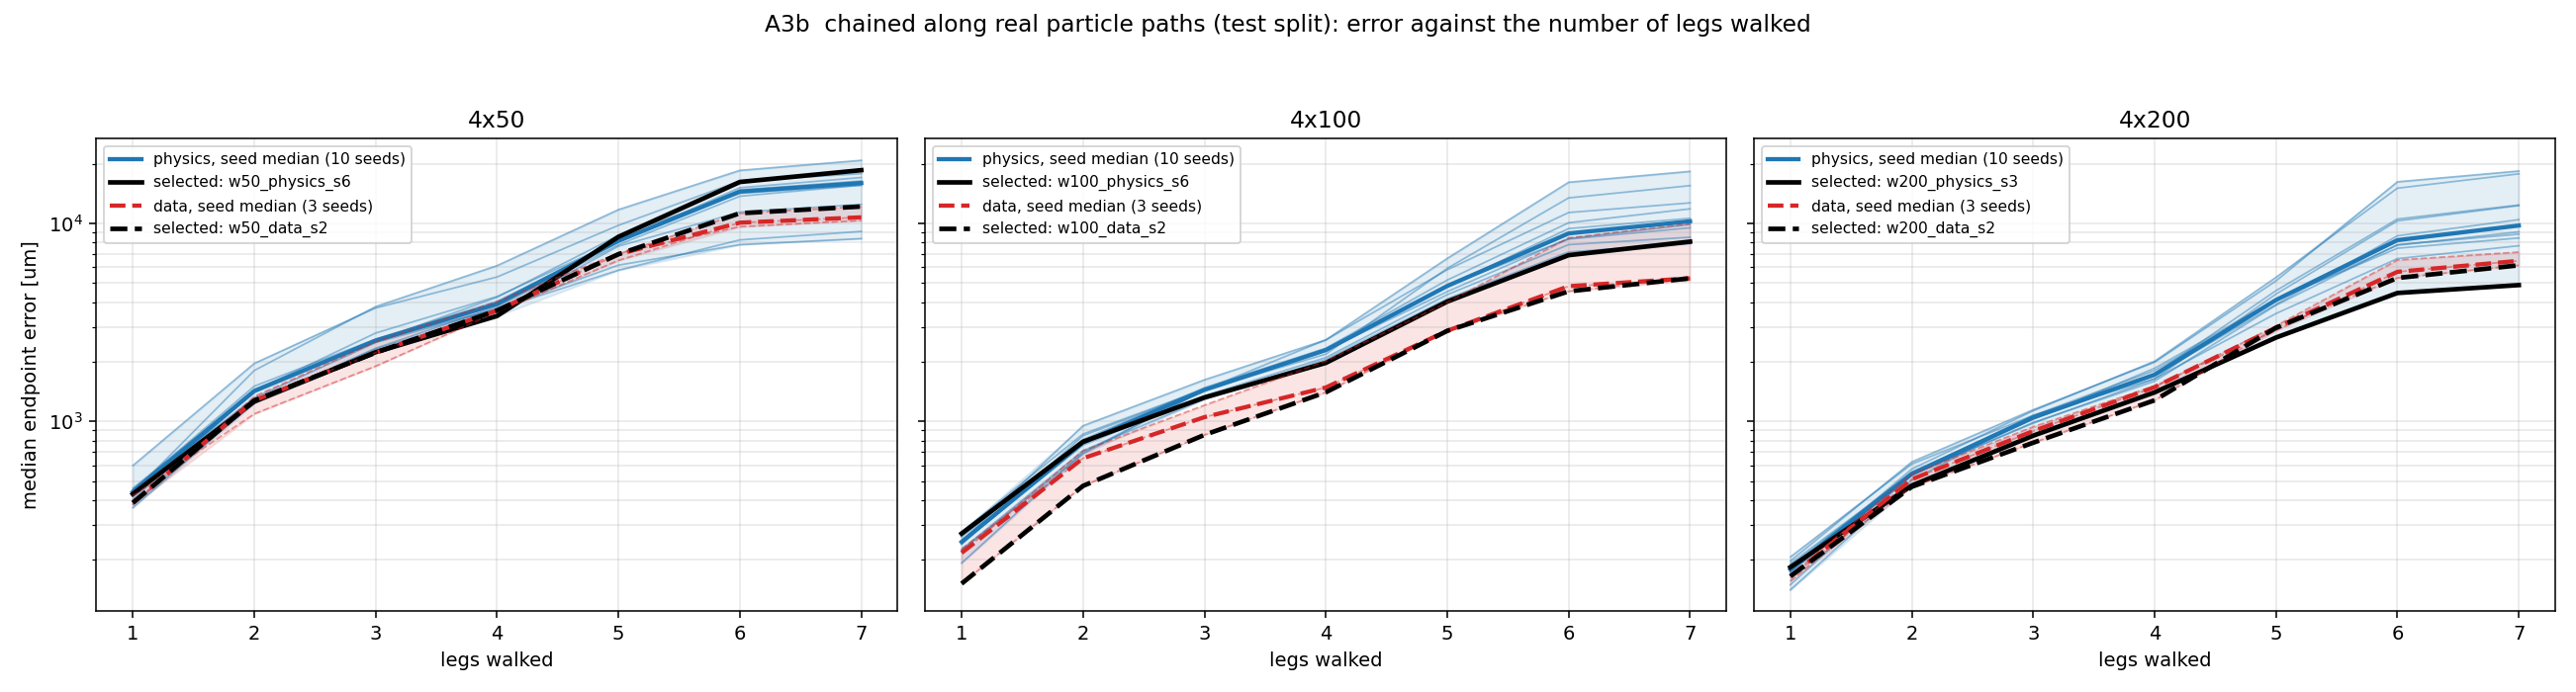
\includegraphics[width=0.92\linewidth]{fig_chains.png}
  \caption{Median endpoint error against the number of legs walked, logarithmic
  vertical axis, for the general network with absolute outputs. Each curve is
  one architecture and loss; bands are the seed spread and the dashed curves are
  the 95th percentiles. The number of contributing particles falls after leg
  four, marked on the axis, because only the longer chains reach those lengths.
  The curves are straight on this axis over the first four legs, which is
  geometric growth: the error roughly doubles per leg rather than growing like
  the square root of the number of legs, the signature of a systematic bias
  rather than independent random errors.}
  \label{fig:chains}
\end{figure}

\subsubsection{Leg D: can a hard step be replaced by two easier ones?}

Leg D, the downstream leg from the first post-magnet plane all the way back to
the collision vertex, is a single backward step with a median length of
$-8.6$ m. No leg D was in the training set, so this is an out-of-training test
by construction. The exact eight-stage scheme itself is only good to $752\um$ on
it, and $216\um$ at $q = 16$; the straight line is $948\mm$.

\begin{table}[tbp]
  \centering
  \caption{Leg D, the giant backward step to the collision vertex, over $2726$
  test particles, in micrometres, median over converged seeds. No leg of this
  geometry was in any training set. Source:
  \texttt{Chained\_legs/results/leg\_d\_reproduction.csv} and
  \texttt{leg\_d\_ceiling\_same\_population.csv}.}
  \label{tab:legd-abs}
  \small
  \begin{tabular}{lrrrrrr}
    \toprule
    & \multicolumn{3}{c}{physics loss} & \multicolumn{3}{c}{data twin} \\
    \cmidrule(lr){2-4}\cmidrule(lr){5-7}
    & $4\times50$ & $4\times100$ & $4\times200$
    & $4\times50$ & $4\times100$ & $4\times200$ \\
    \midrule
    two composite steps & $47{,}353$ & $59{,}416$ & $35{,}034$
                        & $34{,}228$ & $33{,}416$ & $30{,}351$ \\
    the same leg in one giant step & $17{,}947$ & $8778$ & $4563$
                        & $6213$ & $3158$ & $2182$ \\
    \midrule
    \multicolumn{7}{l}{exact $q = 8$ scheme on these legs: $752$;
      $q = 16$: $216$; straight line: $948{,}000$} \\
    \bottomrule
  \end{tabular}
\end{table}

Composite stepping is four to ten times \emph{worse} than the single giant step,
not better, and both are more than an order of magnitude above the scheme's
ceiling. The reason is visible in the first hop, which is longer than any leg in
training and is already $1.5$ to $10\mm$ out. This is not a sign problem: the
network has seen backward steps, since all $1317$ A legs and $490$ of the $1060$
B legs are backward. It is that no leg-D geometry was in training at all, and
the network does not extrapolate to it. It does still beat the straight line by
a factor $100$ to $300$, which is the only thing that can be said for it here.

\subsubsection{The hypothesis this experiment produced}
\label{sec:hypothesis}

I stated the following as a hypothesis before testing it. The general-leg
network is limited by its output parameterisation: it predicts the
\textbf{absolute} state at each stage and at the endpoint, scaled by a single
population-wide constant per component. Four pieces of evidence pointed that
way.

\begin{enumerate}
  \item The output scale on the general-leg dataset is $602\mm$ in $x$ and
  $341\mm$ in $y$, set by the spread of the whole population, which is dominated
  by the $5$ m cross-magnet legs. The physical correction the network must
  produce on a $70\mm$ plane-to-plane leg is the straight-line error on that
  leg, about $7\um$. Resolving a $7\um$ correction on an output whose scale is
  $602\mm$ is asking for a relative precision of one part in $10^{8}$ from a
  network whose loss is normalised at the population scale. On the frozen-leg
  dataset, where the population is one geometry, the corresponding output scale
  is $396\mm$ and the correction is $520\mm$, a completely different regime.
  \item The error is roughly a fixed fraction of the largest step the network
  was trained on, not a fixed fraction of each step: $404$, $2600$ and $300\um$
  on legs whose true corrections span five orders of magnitude, from $6.6\um$ to
  $444\mm$.
  \item On the short legs, where the hypothesis says the error should be a scale
  error rather than an accumulation, the error is flat across the eight Gauss
  nodes. On the long leg, where the bend is genuinely being under-resolved, it
  grows monotonically to the endpoint.
  \item The frozen-leg network, which has exactly the same architecture, loss,
  optimiser and data source but only one geometry and therefore a matched scale,
  is a factor $14$ better on that geometry.
\end{enumerate}

The alternative was capacity, and the second wave at $4 \times 200$ was run to
separate them. Section~\ref{sec:size} predicted that width would buy about $14$
percent over $4 \times 100$ on the frozen leg; on the general-leg dataset it
bought a factor $1.5$ on leg B, leaving the factor $14$ largely intact and the
short legs still an order of magnitude worse than a straight line. That is
consistent with the parameterisation hypothesis and not with the capacity one.

\subsection{The straight-line-residual redesign}
\label{sec:residual}

\textbf{Design.} Exactly one thing changes: what the network is asked to output,
per Eq.~\eqref{eq:residual}, with the per-leg scale of Eq.~\eqref{eq:scale}
built from the bending integral of Eq.~\eqref{eq:bendint}. The dataset is byte
for byte the same population plus three scale arrays per split. The physics
loss, the optimiser protocol, the number of stages, the splits, the momentum
bands, the scorer and the ceilings are all unchanged. Architectures
$4 \times 50$ and $4 \times 100$, label-free seeds $0$ to $9$, supervised seeds
$0$ to $2$: $26$ runs, all $26$ converged.

\begin{figure}[tbp]
  \centering
  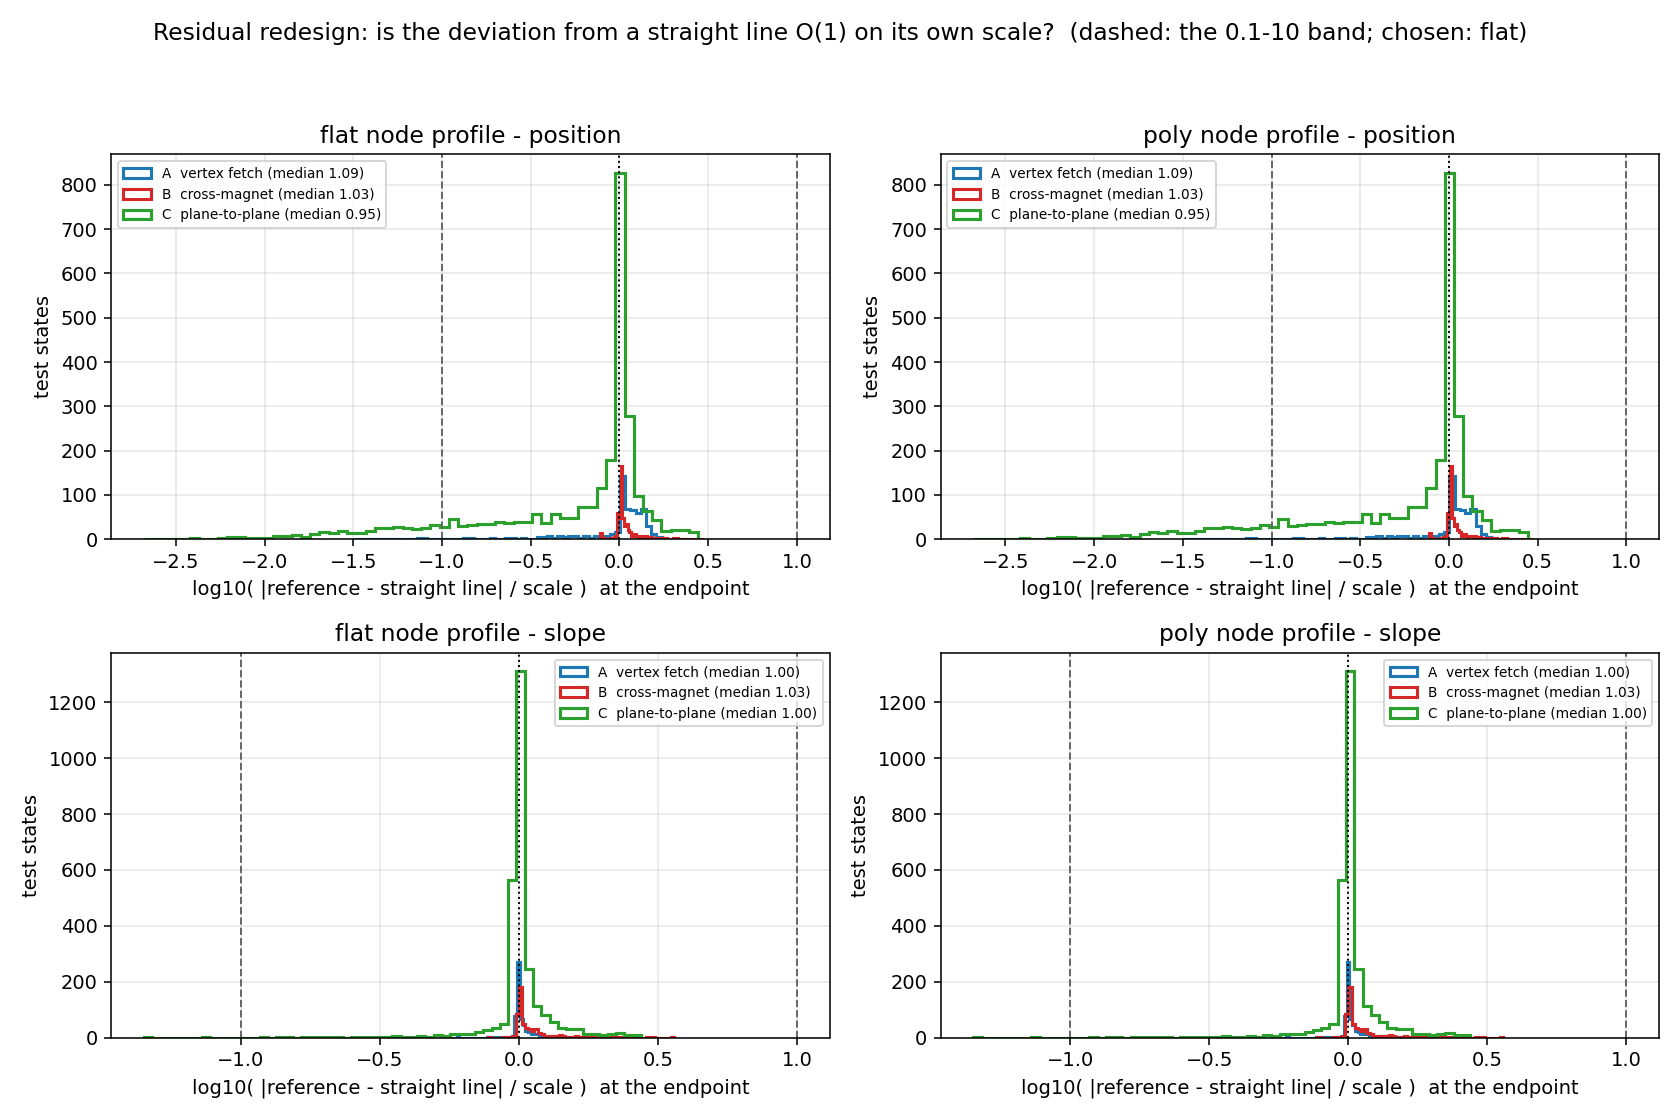
\includegraphics[width=0.62\linewidth]{fig_residual_scale.png}
  \caption{The check that had to pass before any farm time was spent: the
  distribution, by leg type, of the ratio the network will actually have to
  emit, that is the reference deviation from a straight line divided by the
  label-free scale of Eq.~\eqref{eq:scale}. The two node profiles considered are
  shown side by side, flat and polynomial. The rule, fixed before looking, was
  to take flat unless its endpoint medians fell outside $0.1$ to $10$ on some
  leg while the polynomial profile's did not. The medians are $1.09$, $1.03$ and
  $0.95$ on legs A, B and C for both profiles, so the rule selects flat. The
  same label-free expression lands within ten percent of the truth on a $341\mm$
  backward vertex fetch, a $5.2$ m magnet crossing and a $70\mm$ sensor hop,
  which is the $O(1)$ requirement the redesign was built around.}
  \label{fig:residualscale}
\end{figure}

\paragraph{The initialisation check.}
Before the runs, \texttt{train\_residual.py --init-check} verified the algebra at
$4 \times 100$, seed $0$, on the $7935$ training states: the straight-line term
agrees with an independent construction to $4.5 \times 10^{-13}\mm$; zeroing the
last layer makes the output minus the straight line exactly $0.0\mm$; at the
shared trainer's own initialisation the raw network output has median $0.057$
and maximum $0.34$ in units of the residual scale, which is $0.51\um$ at the
median endpoint; and both losses and their maximum gradients are finite. The
last layer is \emph{not} zeroed for the real runs, because a zero last layer
makes every earlier layer's gradient exactly zero on the first step; zeroing is
used only as the algebra check. The consequence is worth stating: an
\emph{untrained} residual network already scores $15.5\um$ on the whole test
split, against $16.1\um$ for a straight line, where the converged
absolute-output networks scored about $300\um$.

\paragraph{The optimisation got easier, not just the answer better.}
The residual runs stall sooner, $40$ to $64$ restarts against $84$ to $121$ at
the same width, at a physics loss an order of magnitude lower,
$9 \times 10^{-7}$ against $1.8 \times 10^{-5}$ at $4 \times 100$ seed $0$. Only
three of the $26$ runs needed the resubmission treatment, against $20$ of the
first $26$ in the absolute-output wave.

\begin{table}[tbp]
  \centering
  \caption{The residual redesign against the absolute-output design, by leg
  type. Test-split median endpoint error in micrometres, median over seeds, with
  the seed range in brackets. The residual $4\times50$ ranges, omitted for
  width, are $3$--$6$, $945$--$1627$ and $1$--$1$. Every column here was
  re-scored in one pass on the same test states by
  \texttt{aggregate\_residual.py}. Source:
  \texttt{General\_leg\_network/results/by\_leg\_residual.csv}.}
  \label{tab:residual}
  \footnotesize
  \setlength{\tabcolsep}{3pt}
  \begin{tabular}{lrrrrrrr}
    \toprule
    & \multicolumn{2}{c}{absolute, physics} & \multicolumn{2}{c}{residual, physics}
    & resid. & & \\
    \cmidrule(lr){2-3}\cmidrule(lr){4-5}
    leg & $4{\times}100$ & $4{\times}200$ & $4{\times}100$ & $4{\times}50$
        & twin & straight & ceiling \\
    \midrule
    A vertex fetch  & $404$ [$286$--$538$]   & $229$ [$201$--$277$]
                    & $\mathbf{4.4}$ [$2$--$6$] & $4.1$
                    & $0.06$ & $10.9$ & $0.0013$ \\
    B cross-magnet  & $2600$ [$2106$--$3152$] & $1740$ [$1632$--$2154$]
                    & $\mathbf{1026}$ [$878$--$1209$] & $1136$
                    & $512$ & $444{,}075$ & $46.4$ \\
    C plane-to-plane& $300$ [$252$--$335$]   & $213$ [$165$--$235$]
                    & $\mathbf{1.6}$ [$1$--$2$] & $1.2$
                    & $0.01$ & $6.6$ & $5.8\times10^{-7}$ \\
    \bottomrule
  \end{tabular}
\end{table}

\begin{table}[tbp]
  \centering
  \caption{Whole test split, all leg types pooled, median over seeds, in
  micrometres. The straight line on this split is $16.1\um$. The
  absolute-output design never beat it at any width; the residual design beats
  it by a factor $7.6$ with the physics loss and $410$ with the twin, and a
  $4 \times 50$ residual network beats a $4 \times 200$ absolute-output network
  by a factor $129$. Source:
  \texttt{General\_leg\_network/results/residual\_summary.csv}.}
  \label{tab:residual-split}
  \small
  \begin{tabular}{lrrrrrr}
    \toprule
    & \multicolumn{3}{c}{physics loss} & \multicolumn{3}{c}{data twin} \\
    \cmidrule(lr){2-4}\cmidrule(lr){5-7}
    output design & $4\times50$ & $4\times100$ & $4\times200$
                  & $4\times50$ & $4\times100$ & $4\times200$ \\
    \midrule
    absolute states & $721$ & $397$ & $273$ & $637$ & $321$ & $237$ \\
    straight-line residual & $\mathbf{2.12}$ & $\mathbf{2.64}$ & not run
                           & $\mathbf{0.06}$ & $\mathbf{0.04}$ & not run \\
    \bottomrule
  \end{tabular}
\end{table}

Read across Table~\ref{tab:residual}.

\begin{enumerate}
  \item \textbf{The two short legs are transformed.} Leg A goes $404 \to 4.4\um$,
  a factor $92$; leg C goes $300 \to 1.6\um$, a factor $190$. Both now sit
  \emph{below} the straight line, by a factor $2.5$ on A and $4$ on C, where the
  absolute-output design sat thirty to fifty times above it, which is the
  hypothesis's own prediction.
  \item \textbf{The cross-magnet leg improves by a factor $2.5$}, $2600 \to
  1026\um$. Real, but an order of magnitude short of the same transformation.
  Leg B is the one leg where the absolute output scale was roughly right, so it
  had least to gain. The redesign fixed a conditioning problem, and what is left
  on leg B is not a conditioning problem.
  \item \textbf{Width has stopped mattering} on legs A and C: $4 \times 50$ and
  $4 \times 100$ are within $20$ percent of each other, and on both legs the
  narrower network is the better of the two. The absolute-output verdict read
  the width trend as evidence that width was the binding constraint. It was
  never width. It was the parameterisation.
  \item \textbf{The data twin is extraordinary on the short legs}, $0.06\um$ on
  A and $0.01\um$ on C, four orders of magnitude better than the
  absolute-output twin on each, and still twice as good as the physics loss on
  leg B, $512$ against $1026\um$, where it is a factor $11$ above the ceiling.
  The gap between the two losses has widened in relative terms on the easy legs
  and narrowed on the hard one.
  \item \textbf{Distance to the ceiling, which is the honest scorecard.} Against
  the exact $q = 8$ scheme on the same states, the residual $4 \times 100$
  physics network is $3400$ times above the ceiling on leg A, $22$ times on leg
  B and $2.7 \times 10^{6}$ times on leg C. The absolute-output factors were
  $310{,}000$, $56$ and $5 \times 10^{8}$. So the gap closed by two orders of
  magnitude on A and C and by a factor $2.5$ on B, but the network is nowhere
  near the scheme it is solving on any leg, and on the short legs the scheme is
  so nearly exact that no network is going to reach it.
\end{enumerate}

\begin{figure}[tbp]
  \centering
  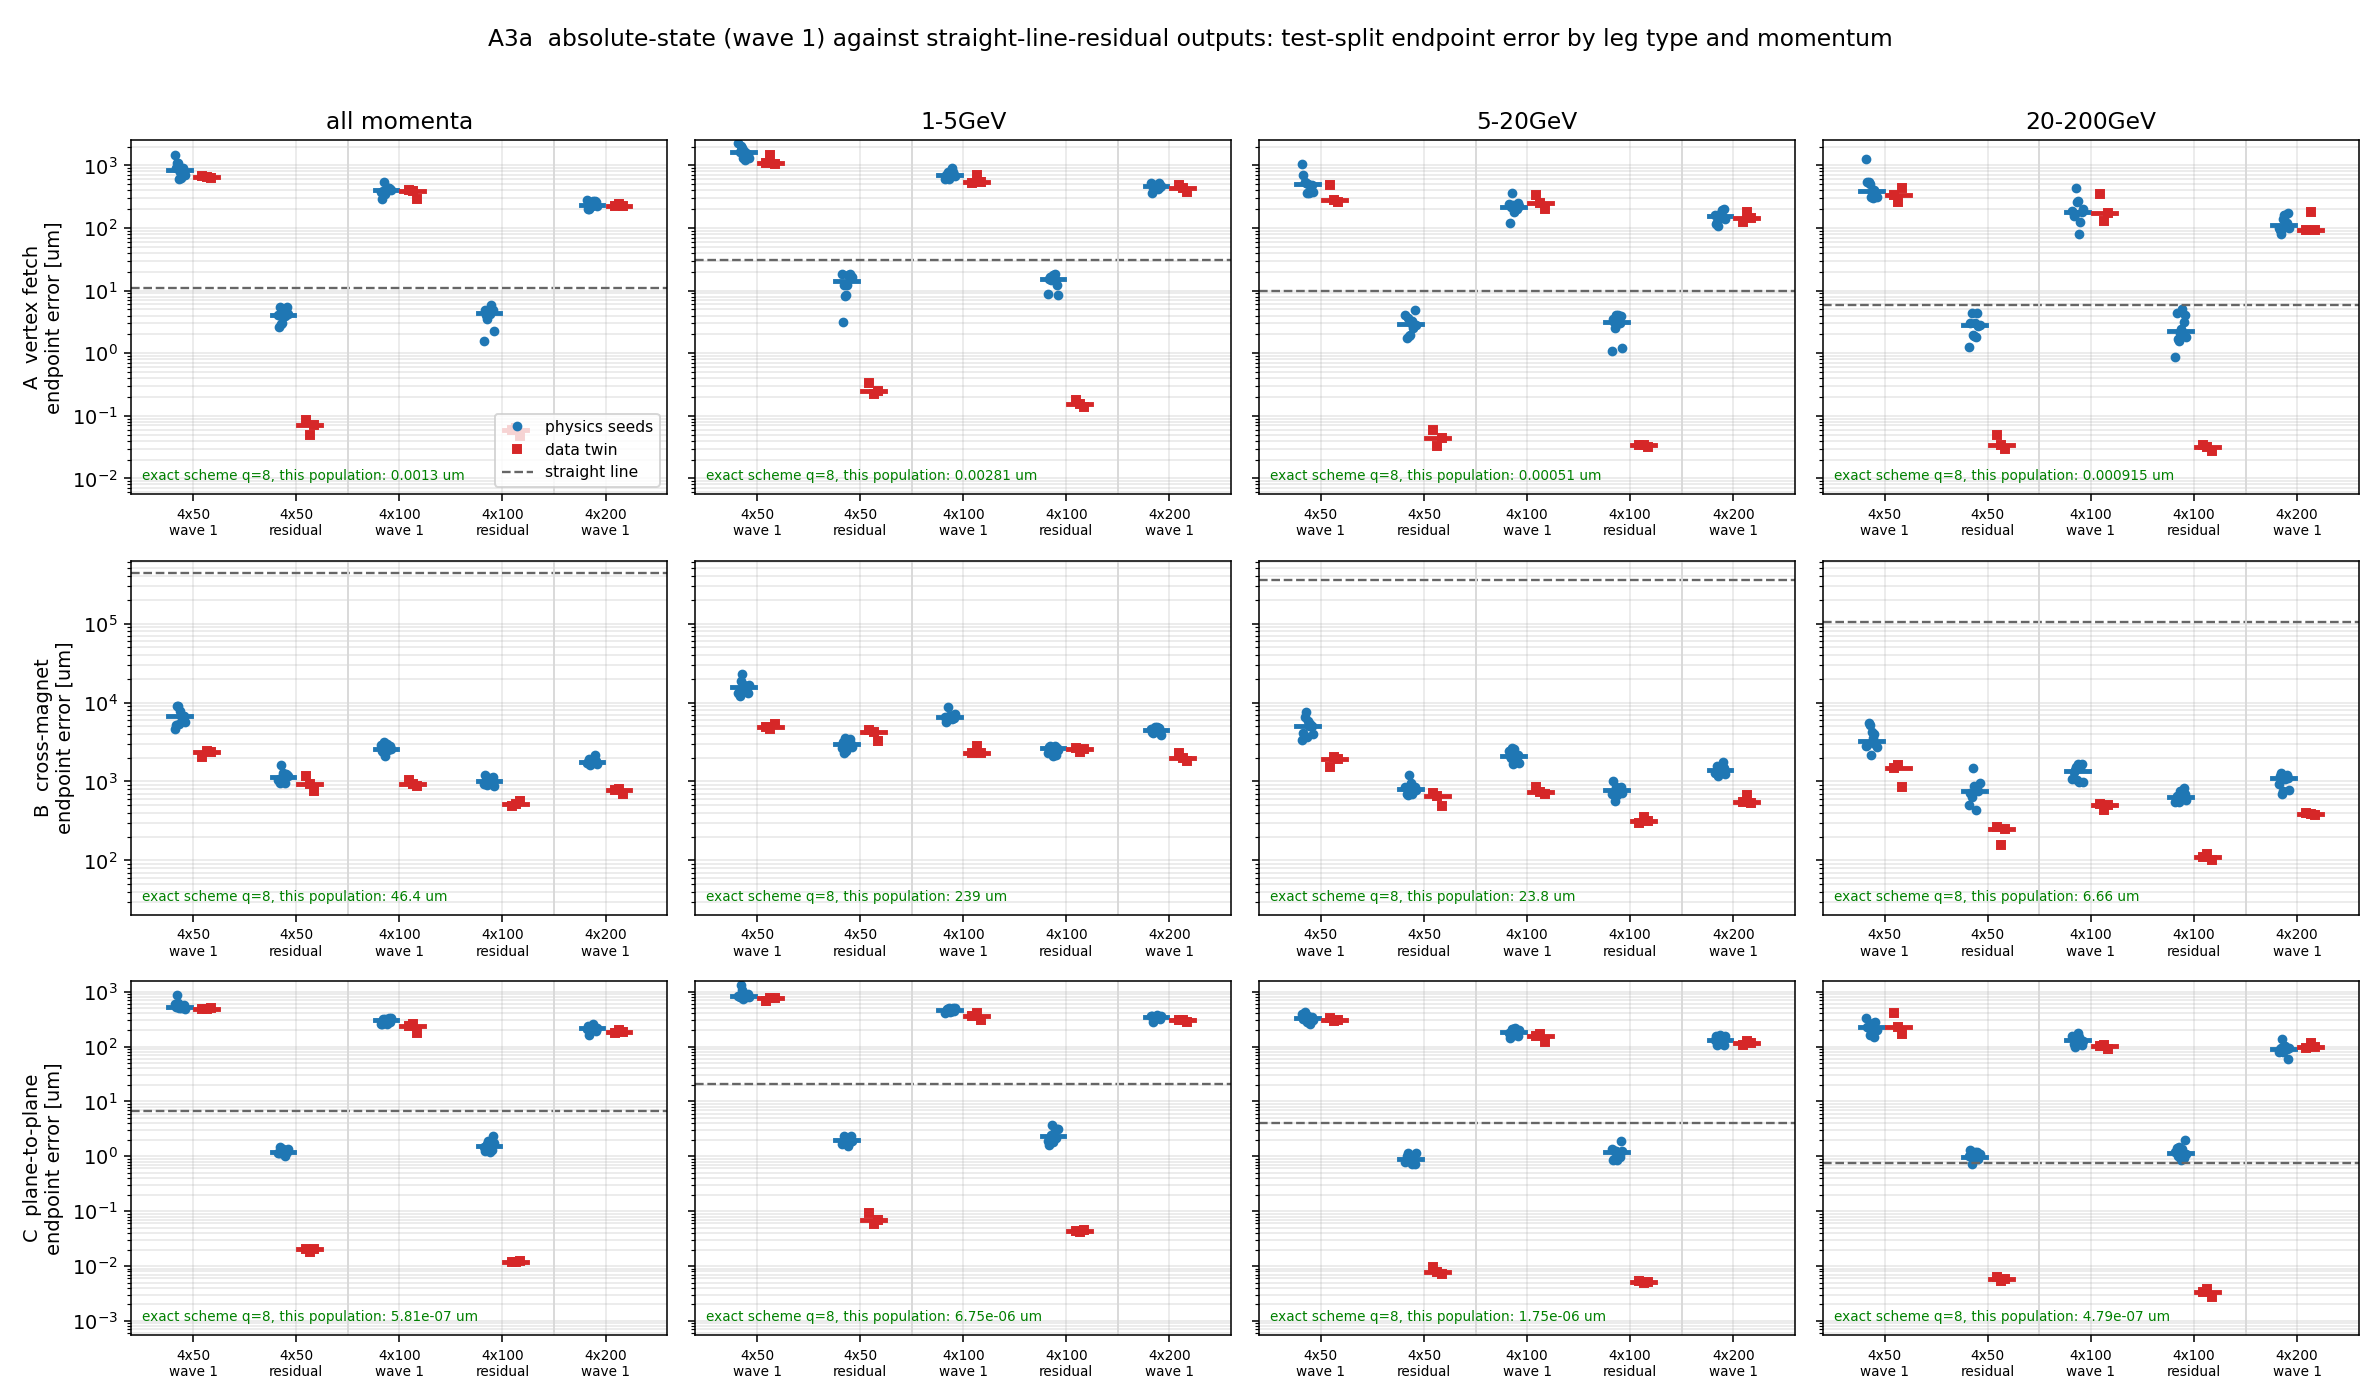
\includegraphics[width=0.82\linewidth]{fig_residual_legs.png}
  \caption{The same layout as Figure~\ref{fig:generallegs}, with the residual
  arm added. Rows are leg types A, B and C, columns are momentum bands, and the
  vertical axis is logarithmic. The absolute-output seeds are the upper cloud in
  each panel and the residual seeds the lower one, with the straight-line
  baseline as a dashed grey line and the exact-scheme ceiling annotated. On the
  top and bottom rows the residual cloud crosses from above the straight line to
  below it, which is the whole point of the redesign; on the middle row it moves
  down by a factor $2.5$ and stays well above both the ceiling and its own
  supervised twin. The improvement on legs A and C is uniform in momentum, a
  factor $46$ to $200$ in every band, so it is not an artefact of the momentum
  mix. The one cell where the residual network is still worse than a straight
  line is plane-to-plane at $20$ to $200$ GeV, $1.2\um$ against $0.74\um$: a
  stiff $70\mm$ hop is so nearly straight that there is essentially nothing to
  predict, and the network's own noise floor is above the thing it is
  correcting.}
  \label{fig:residuallegs}
\end{figure}

\subsubsection{Where the error lives inside the step}

\begin{table}[tbp]
  \centering
  \caption{Median position error at each of the eight Gauss nodes and at the
  endpoint, test split, $4 \times 100$ physics loss, median over seeds, in
  micrometres. The absolute-output error on legs A and C is flat across the
  step, which is the signature of a scale error the network cannot resolve. The
  residual error instead grows monotonically from the first node to the
  endpoint, by a factor $50$ to $70$ on A and C: the flat offset is gone and
  what is left is the honest accumulation of an under-resolved bend. Leg B kept
  its monotonic growth and simply scaled down by $2.5$. Source:
  \texttt{General\_leg\_network/results/stage\_errors\_residual.csv}.}
  \label{tab:stage-errors}
  \small
  \begin{tabular}{lrrrrrrrrr}
    \toprule
    & node 1 & 2 & 3 & 4 & 5 & 6 & 7 & 8 & endpoint \\
    \midrule
    absolute, leg A & $365$ & $340$ & $353$ & $320$ & $312$ & $408$ & $349$ & $381$ & $404$ \\
    residual, leg A & $0.06$ & $0.10$ & $0.43$ & $1.01$ & $1.74$ & $2.81$ & $3.64$ & $4.34$ & $4.42$ \\
    \midrule
    absolute, leg C & $289$ & $240$ & $249$ & $270$ & $260$ & $271$ & $268$ & $278$ & $300$ \\
    residual, leg C & $0.03$ & $0.05$ & $0.29$ & $0.65$ & $0.88$ & $1.12$ & $1.34$ & $1.52$ & $1.57$ \\
    \midrule
    absolute, leg B & $987$ & $905$ & $1054$ & $1436$ & $1907$ & $2326$ & $2536$ & $2519$ & $2600$ \\
    residual, leg B & $108$ & $143$ & $277$ & $456$ & $616$ & $812$ & $924$ & $988$ & $1026$ \\
    \bottomrule
  \end{tabular}
\end{table}

Table~\ref{tab:stage-errors} is the clearest single piece of evidence that the
diagnosis of Section~\ref{sec:hypothesis} was right.

\begin{figure}[tbp]
  \centering
  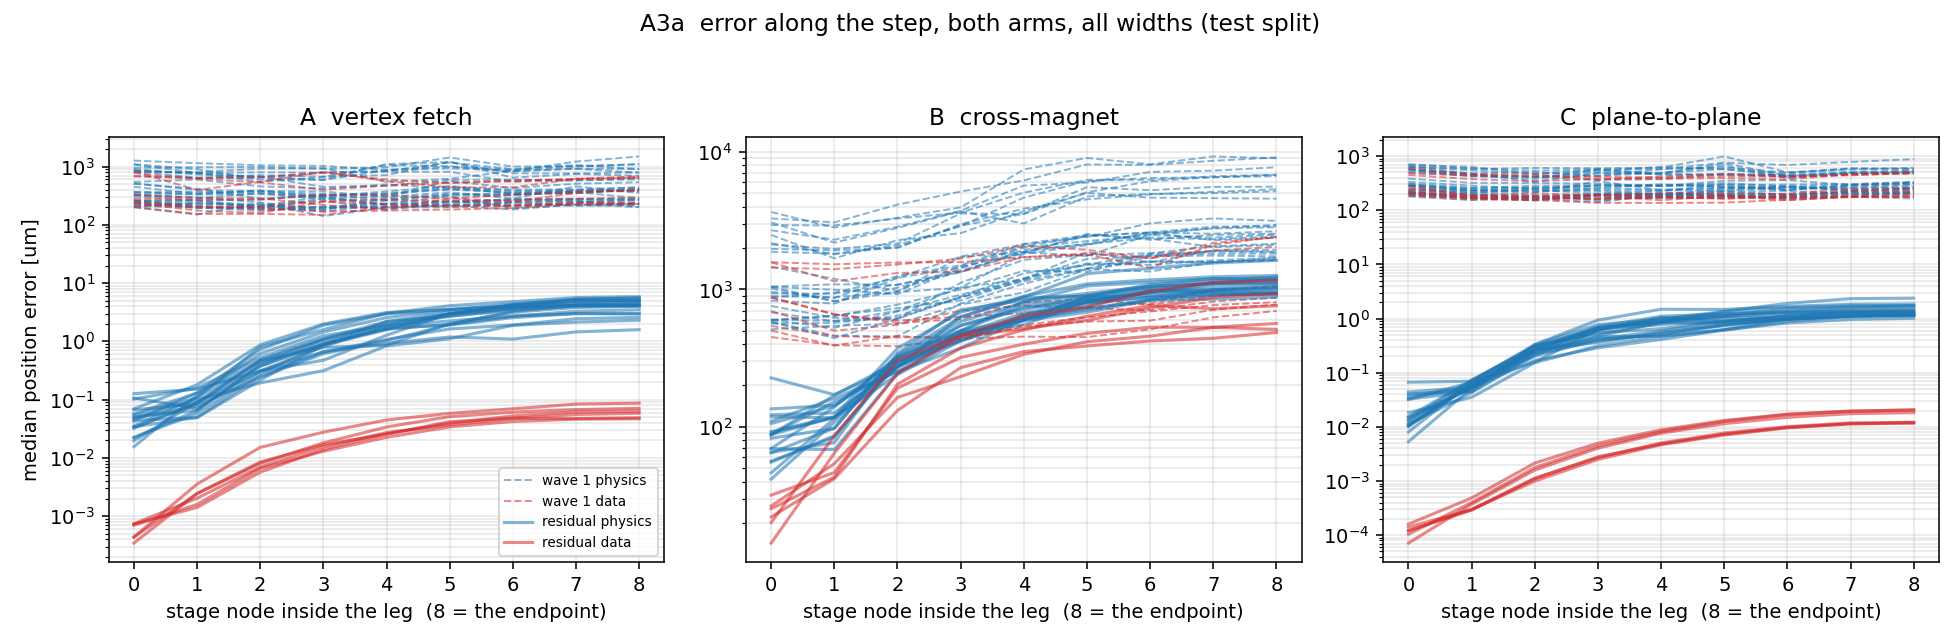
\includegraphics[width=0.95\linewidth]{fig_residual_stages.png}
  \caption{The error along the step, both output designs, one panel per leg
  type. The horizontal axis is the eight Gauss--Legendre nodes and then the
  endpoint; the vertical axis is the median position error in micrometres, on a
  logarithmic scale. The absolute-output curves on legs A and C are flat, the
  residual curves rise steeply from a very small first node. A flat profile
  means the error is present before any physics has happened and is therefore an
  offset; a rising profile means it is accumulated along the step.}
  \label{fig:residualstages}
\end{figure}

\subsubsection{What did not improve: the tails}
\label{sec:tails}

\begin{table}[tbp]
  \centering
  \caption{The 95th percentile of the endpoint error, all momenta,
  $4 \times 100$, in micrometres. Leg C's tail improves with its median by a
  factor $10$ to $70$. Legs A and B do not, and the residual twin's tail on leg
  A is twice the absolute-output twin's. Source:
  \texttt{General\_leg\_network/results/by\_leg\_residual.csv}, column
  \texttt{endpoint\_p95\_um}.}
  \label{tab:tails}
  \small
  \begin{tabular}{lrrrr}
    \toprule
    leg & absolute, physics & residual, physics & absolute, twin & residual, twin \\
    \midrule
    A & $30{,}693$ & $23{,}640$ & $10{,}445$ & $20{,}128$ \\
    B & $41{,}542$ & $27{,}080$ & $18{,}395$ & $17{,}425$ \\
    C & $2862$     & $\mathbf{292}$ & $2193$ & $\mathbf{32}$ \\
    \bottomrule
  \end{tabular}
\end{table}

A small population of states got worse while the bulk got thousands of times
better. Those are the soft tracks that bend hardest. The residual scale of
Eq.~\eqref{eq:scale} is a first-order estimate, and where the true deviation is
many times that estimate the network is back to writing down a large number.
Fixing the median did not fix the tail, and the tail is what an extrapolator
with a bounded time budget actually has to survive.

\subsubsection{Chaining the residual networks}

\begin{table}[tbp]
  \centering
  \caption{The residual networks chained along the same real particle paths, and
  the absolute-output networks for comparison. Median endpoint error against the
  reference path, test split, in micrometres. Source:
  \texttt{Chained\_legs/results/chain\_summary\_residual.csv}.}
  \label{tab:chains-residual}
  \footnotesize
  \setlength{\tabcolsep}{3pt}
  \begin{tabular}{crrrrrr}
    \toprule
    legs & \multicolumn{2}{c}{absolute $4{\times}100$}
         & \multicolumn{3}{c}{residual} & \\
    \cmidrule(lr){2-3}\cmidrule(lr){4-6}
    walked & physics & twin & $4{\times}100$ & $4{\times}100$ twin
           & $4{\times}50$ & particles \\
    \midrule
    $1$ & $246$      & $217$  & $\mathbf{1.2}$  & $\mathbf{0.01}$ & $1.1$  & $4563$ \\
    $2$ & $783$      & $652$  & $\mathbf{60}$   & $\mathbf{2.7}$  & $59$   & $4563$ \\
    $3$ & $1443$     & $1051$ & $\mathbf{281}$  & $\mathbf{32}$   & $261$  & $4563$ \\
    $4$ & $2293$     & $1484$ & $\mathbf{572}$  & $\mathbf{118}$  & $568$  & $4563$ \\
    $5$ & $4831$     & $2869$ & $1750$          & $471$           & $1919$ & $2914$ \\
    $6$ & $8904$     & $4820$ & $3804$          & $1052$          & $3973$ & $1481$ \\
    $7$ & $10{,}248$ & $5284$ & $4492$          & $1259$          & $4739$ & $853$ \\
    \bottomrule
  \end{tabular}
\end{table}

Two things are true at once and they pull in opposite directions.

\textbf{The chain is better everywhere.} After four legs the residual network is
$4.0$ times better than the absolute-output one with the physics loss, $572$
against $2293\um$, and $12.6$ times better with the twin, $118$ against
$1484\um$. Over a full seven-leg path it is still $2.3$ and $4.2$ times better.
The 95th percentile improves by the same factor at every step, $13.1\mm$ against
$38.6\mm$ at leg four, so this is the whole distribution moving and not the
median alone.

\textbf{But the compounding got worse.} The step-to-step growth ratios at
$4 \times 100$ with the physics loss are $48.6$, $4.67$, $2.04$, $3.06$, $2.17$,
$1.18$, against $3.18$, $1.84$, $1.59$, $2.11$, $1.84$, $1.15$ for the
absolute-output design. The residual network starts two hundred times lower,
$1.2\um$, which is essentially its own one-step plane-to-plane number, and then
multiplies by $49$ on the second leg and $4.7$ on the third before settling into
the same factor of two per leg. By leg four the two curves are only a factor $4$
apart and by leg seven a factor $2.3$.

The reason is visible in the one-step table. A chain's early legs are short
plane-to-plane hops, where the residual network is at $1.6\um$, and its later
legs include the cross-magnet crossing, where it is at $1026\um$, the leg the
redesign barely improved. The chain error is therefore dominated, after two or
three steps, by the one leg that did not get better. The redesign bought a much
better start, not a slower compounding. Nothing diverges and nothing saturates.

Seed selection survives the change. Ranking physics seeds by the median chain
error after four legs on validation and reading them out on test gives rank
correlations of $0.98$ at $4 \times 50$ and $0.90$ at $4 \times 100$, so a seed
can still be chosen on validation data without touching test. The cheap
alternative improves but is still not usable: the one-step validation error now
correlates with the chained test error at $0.72$ at $4 \times 100$ and $0.35$ at
$4 \times 50$, where in the absolute-output arm it carried no information at all
at $0.08$. That is consistent with the picture above, since once the one-step
number is dominated by the same leg that dominates the chain the two start to
agree, but $0.72$ over ten seeds is not enough to select on, and the ten seeds
differ by $60$ percent in chained error at fixed architecture, $487$ to $783\um$
at $4 \times 100$.

\subsubsection{Leg D under the residual parameterisation}

\begin{table}[tbp]
  \centering
  \caption{Leg D, the giant backward step to the collision vertex, under the
  residual parameterisation, over the same $2726$ test particles, in
  micrometres. The stored label agrees with a fresh reference pass to
  $0.045\um$. Source:
  \texttt{Chained\_legs/results/leg\_d\_residual.csv}.}
  \label{tab:legd-residual}
  \footnotesize
  \setlength{\tabcolsep}{3pt}
  \begin{tabular}{lrrrrr}
    \toprule
    & \multicolumn{2}{c}{absolute $4{\times}100$}
    & \multicolumn{3}{c}{residual} \\
    \cmidrule(lr){2-3}\cmidrule(lr){4-6}
    & physics & twin & $4{\times}100$ & $4{\times}100$ twin & $4{\times}50$ \\
    \midrule
    two composite steps & $59{,}416$ & $33{,}416$ & $\mathbf{4252}$ & $\mathbf{2374}$ & $4768$ \\
    one giant step      & $8778$     & $3158$     & $\mathbf{3749}$ & $\mathbf{2213}$ & $3806$ \\
    \midrule
    \multicolumn{6}{l}{exact $q = 8$ scheme on these legs: $752$; $q = 16$:
      $216$; straight line: $948{,}000$} \\
    \bottomrule
  \end{tabular}
\end{table}

Three readings. The composite improves by a factor $14$, from $59.4$ to
$4.3\mm$ at $4 \times 100$ with the physics loss, far more than the single giant
step's factor $2.3$: the composite's first hop is a $-6.4$ m backward step,
longer than any B leg, and it went from $4.1$ to $1.5\mm$, while its second hop
is a vertex-fetch-like leg, exactly where the residual arm gained a factor $92$
one-step. Walking the leg in two steps is still worse than taking it in one,
$4252$ against $3749\um$, but the gap has closed from a factor $6.8$ to a factor
$1.13$, so the earlier conclusion that composite stepping actively destroys
accuracy is now only marginally true. And both remain five times the exact
scheme's own ceiling of $752\um$ on this geometry, with the 95th percentile
barely moved, $142\mm$ against $149\mm$: the soft-track tail that dominates leg
D is untouched.

\begin{figure}[tbp]
  \centering
  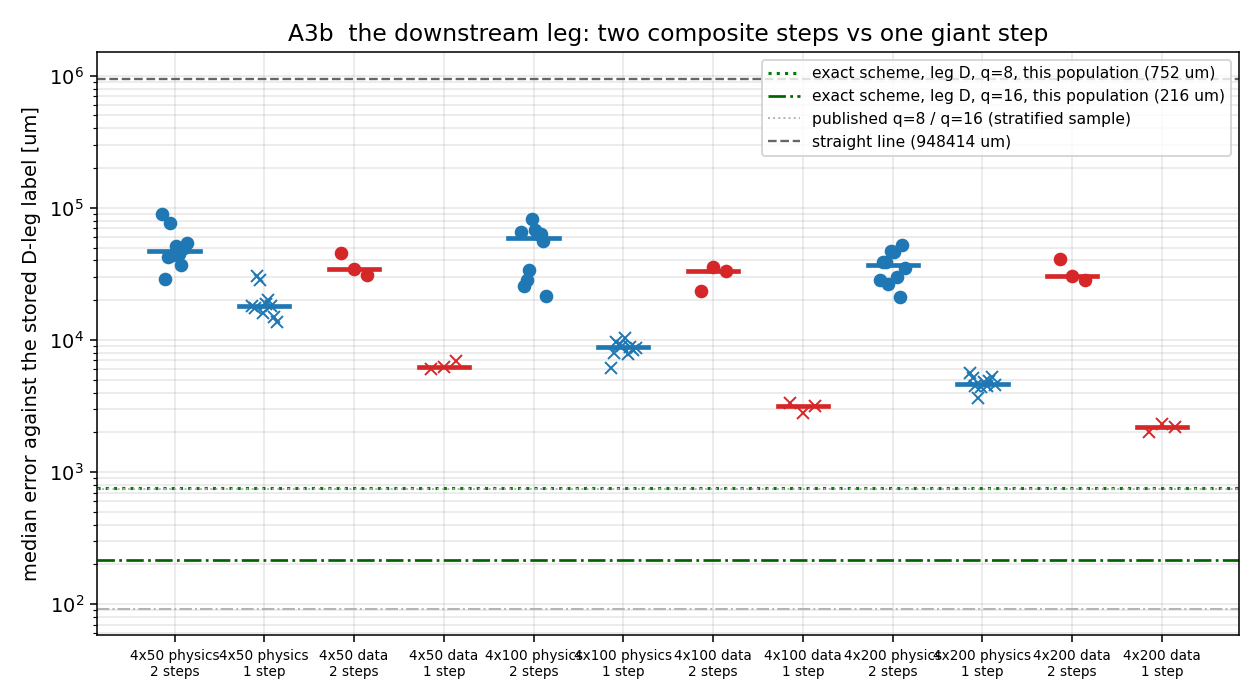
\includegraphics[width=0.68\linewidth]{fig_leg_d.png}
  \caption{Leg D, the single backward step of median length $-8.6$ m from the
  first post-magnet plane to the collision vertex, a geometry that appears in no
  training set. Left: the distribution of endpoint errors for the composite
  route and for the single giant step, on a logarithmic axis, with the exact
  scheme's ceiling and the straight-line baseline marked. Right: the same
  comparison against track momentum. The composite route, which was supposed to
  replace a hard step by two easier ones, is worse than the single step at every
  momentum, because its first hop is longer than any leg in training.}
  \label{fig:legd}
\end{figure}

\begin{figure}[tbp]
  \centering
  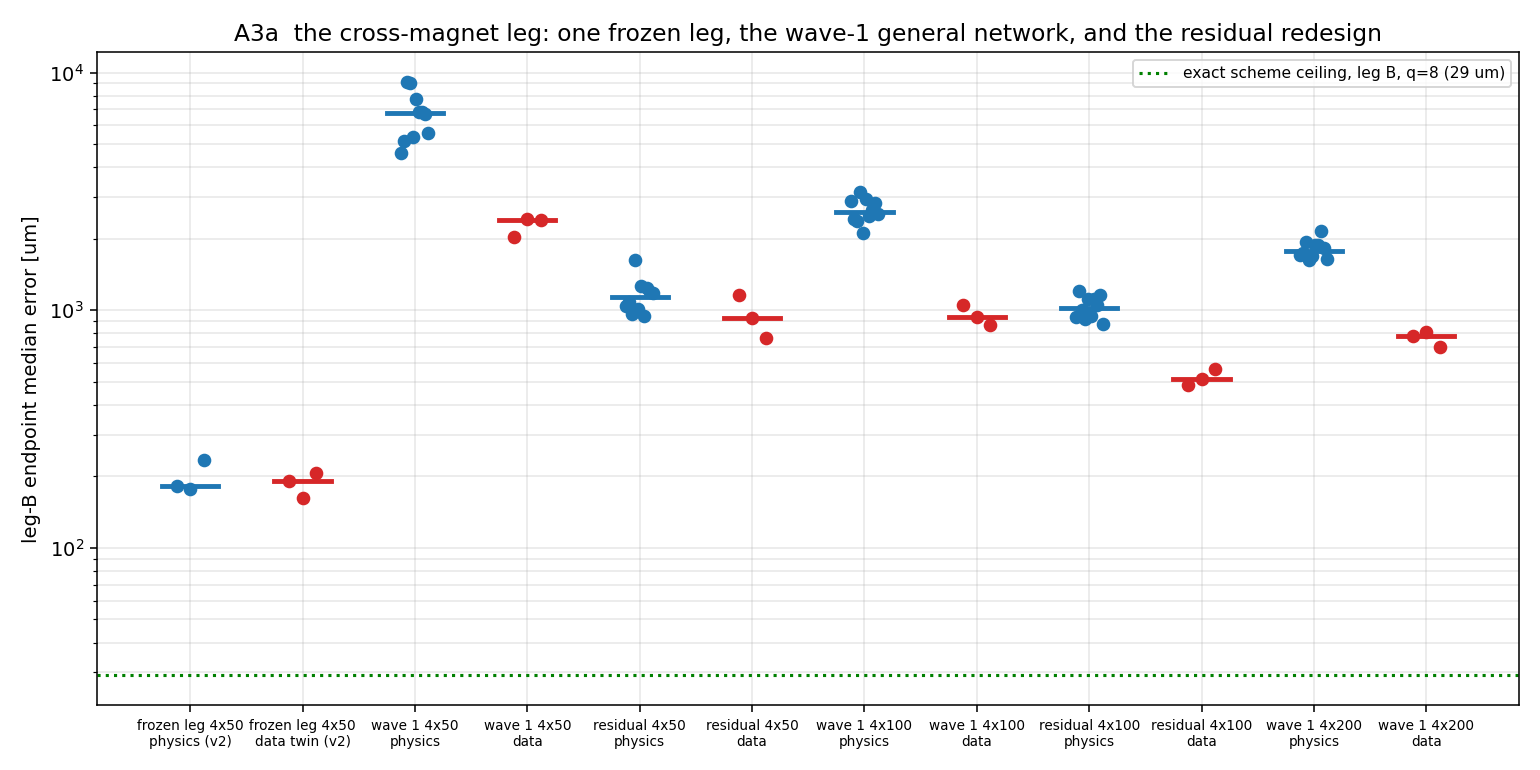
\includegraphics[width=0.62\linewidth]{fig_frozen_vs_general.png}
  \caption{The cross-magnet leg across all three designs on one axis: the
  frozen-leg network, which trains on that geometry alone; the general network
  with absolute outputs; and the general network with the straight-line-residual
  parameterisation. The exact-scheme ceiling on each population and the
  straight-line baseline are drawn. Making the leg an input costs a factor $14$
  against the frozen-leg network, and the residual redesign recovers a factor
  $2.5$ of it. This gap, and not the output scale, is what
  Section~\ref{sec:outlook} proposes to attack next.}
  \label{fig:frozenvsgeneral}
\end{figure}

\subsection{The assembled verdict}
\label{sec:verdict}

Table~\ref{tab:verdict} puts every measurement on one page. All entries are
test-split median endpoint errors in micrometres, defined as in
Section~\ref{sec:metrics}, with the range across seeds in brackets where more
than one seed contributes. The frozen leg is the cross-magnet crossing from
$z = 2648\mm$ to $z = 7826\mm$ with $q = 8$ stages.

\begin{table}[tbp]
  \centering
  \caption{The whole programme on one page. Test-split median endpoint error in
  micrometres. Columns 1 and 2 are the frozen cross-magnet leg at two network
  sizes; column 3 is the same leg on the reversed magnet polarity; columns 4 and
  5 are the single network serving legs A, B and C, quoted per leg, under the
  two output parameterisations; column 6 is that network walked four legs along
  a real particle path. Each column's ceiling is measured on that column's own
  population.}
  \label{tab:verdict}
  \scriptsize
  \setlength{\tabcolsep}{3pt}
  \begin{tabular}{lrrrccr}
    \toprule
    & \multicolumn{2}{c}{frozen leg} & magnet up
    & \multicolumn{2}{c}{one network, legs A / B / C, $4\times100$}
    & chained \\
    \cmidrule(lr){2-3}\cmidrule(lr){5-6}
    & $4\times50$ & $4\times200$ & $4\times50$
    & absolute & residual & 4 legs \\
    \midrule
    exact scheme (ceiling)
      & $23$ & $23$ & $22$
      & $0.0013$ / $46$ / $6\!\times\!10^{-7}$
      & $0.0013$ / $46$ / $6\!\times\!10^{-7}$
      & n.m. \\
    network, physics loss
      & $222$ & $115$ & $229$
      & $404$ / $2600$ / $300$
      & $4.4$ / $1026$ / $1.6$
      & $572$ \\
    network, data twin
      & $192$ & $128$ & $204$
      & $385$ / $933$ / $235$
      & $0.06$ / $512$ / $0.01$
      & $118$ \\
    straight line
      & $520{,}444$ & $520{,}444$ & $525{,}184$
      & $10.9$ / $444{,}075$ / $6.6$
      & $10.9$ / $444{,}075$ / $6.6$
      & n.a. \\
    \midrule
    seed range, physics
      & [$165$--$244$] & [$100$--$134$] & [$171$--$296$]
      & 10 seeds & 10 seeds & selected seed \\
    \bottomrule
  \end{tabular}
\end{table}

\paragraph{The cost argument.}
For the same accuracy class, solving the exact eight-stage scheme with a
root-finder takes a median of $44$ residual evaluations per leg, each of which
evaluates the field at all eight stage points, and the number is not known in
advance. The trained network takes \textbf{one forward pass}, with all eight
stage states emitted at once, and its cost is fixed. That ratio, and not the
accuracy, is the argument for the whole exercise: a trigger can schedule a fixed
cost and cannot easily schedule a loop whose trip count depends on the track.

% ===========================================================================
\section{Discussion}
\label{sec:discussion}

\subsection{Question 1, does it work: yes, on every test}

Four measurements answer it, and they are the four the question was written
around.

\textbf{The label-free training is stable.} Across the campaign $232$ runs were
trained and $208$ reached a confirmed stall: all $24$ of the stage sweep, all
$26$ of the general-leg first wave, $12$ of $13$ of the second wave, all $13$ of
the reversed-polarity experiment, all $26$ of the residual redesign, and $96$ of
the $120$ in the architecture grid. The $24$ that did not confirm are all in the
architecture grid, all at width $32$ or depth $6$, and none of them diverged:
they failed the confirmation pass, in which a fresh optimiser moves a small or
deep network again rather than re-stalling. No run blew up.

\textbf{Where the scheme is the limiting factor, the network sits on the
scheme's own error}, $5202$ against $5198\um$ at $q = 2$ and $5371$ against
$5401\um$ at $q = 4$, agreements of $0.1$ and $0.6$ percent
(Table~\ref{tab:stages}). \textbf{Where the network is the limiting factor, the
shortfall is identified}: optimisation and not capacity, by the loss-error rank
correlation of $+0.965$ over $96$ converged runs
(Figure~\ref{fig:lossvserror}). \textbf{At $4 \times 200$ the label-free loss
beats its own supervised twin}, whose median is $12$ percent higher with a wider
seed spread. And \textbf{on a field polarity for which no labels exist anywhere
in the project} it reaches the same floor, $229$ against $222\um$, and sits the
same distance above that polarity's own ceiling (Table~\ref{tab:magnetup}).

\subsection{Question 2, can it be used: the residual design changed the answer}

Under the absolute-output design the answer was mechanically yes and usefully
no. The general network was a factor $14$ worse than the frozen-leg network on
the same kind of leg and worse than a straight line on the two short leg types;
the chained error compounded to $5$ to $10\mm$ over a full path; and composite
stepping made the giant downstream leg worse rather than better.

The residual redesign of Section~\ref{sec:residual} changed three of those four
statements. The short legs went from thirty to fifty times worse than ignoring
the magnet to two to four times better, and they did so uniformly in momentum.
The whole test split went from $274\um$ at the best absolute-output width to
$2.1\um$, against $16.1\um$ for a straight line. The chain improved by a factor
$4$ to $13$ at every length. Composite stepping went from six times worse than
the single giant step to $13$ percent worse. And an untrained residual network,
by construction, already scores $15.5\um$ against the straight line's $16.1\um$,
so the trivial baseline is inside the parameterisation rather than something the
network must rediscover.

\textbf{What is left is one leg.} The cross-magnet crossing inside a shared
network sits at $1026\um$ against a $46\um$ ceiling on its own population, a
factor $22$, and the redesign moved it by only a factor $2.5$. It is not width:
$4 \times 50$ and $4 \times 100$ agree within ten percent on it. It is not the
output scale: leg B is the one leg where the absolute scale was roughly right,
which is precisely why it had least to gain. Three further observations sharpen
the target.

\begin{enumerate}
  \item \textbf{The supervised twin is also stuck}, at $512\um$ on leg B, a
  factor $11$ above the ceiling, while it reaches $0.06$ and $0.01\um$ on the
  other two legs. Whatever limits leg B limits both losses, so it is not a
  property of the label-free objective.
  \item \textbf{Leg B is a minority of the training states.} Only $1060$ of the
  $7935$ training states, $13$ percent, are cross-magnet legs, and $5558$, $70$
  percent, are plane-to-plane hops. Under the absolute parameterisation that did
  not matter, because the population-wide output scale was set by the long legs
  and they dominated the loss anyway. Under the residual parameterisation every
  leg is $O(1)$ by construction, so every leg now contributes comparably to the
  loss, and the gradient is dominated by the plane-to-plane majority. The
  redesign fixed the conditioning and, in doing so, handed the optimisation
  budget to the easy legs.
  \item \textbf{The error on leg B grows monotonically along the step} in both
  designs, roughly a factor ten from the first node to the endpoint, which is
  the signature of a bend that is being under-resolved rather than of an offset.
\end{enumerate}

Those three together make the cross-magnet leg inside a shared network the
binding constraint on the product, and they suggest the remedy is a change to
what the network is asked to carry rather than to how much of it there is.

\subsection{Caveats, stated plainly}

\begin{itemize}
  \item \textbf{The tails did not improve with the medians.} On legs A and B the
  95th percentile of the residual arm is no better than the absolute-output
  arm's, and the residual twin's tail on leg A is twice as large,
  Table~\ref{tab:tails}. The population responsible is the soft, hard-bending
  tracks for which the first-order scale of Eq.~\eqref{eq:scale} is a poor
  estimate. An extrapolator with a bounded time budget has to survive its tail,
  not its median, so this is a real limitation and not a presentational one.
  \item \textbf{One unconverged seed.} In the general-leg second wave one of the ten
  label-free seeds at the widest architecture stopped at $111$ restarts, far
  short of its $400$-restart cap, in the re-stalled-but-still-moving state
  described below. It was resubmitted but the farm queue was long, so it is reported
  unconverged and excluded from every median. It ranks third on the validation
  chain and does not affect the seed selection.
  \item \textbf{Ceilings are population-dependent.} The $29\um$ figure published
  in July was measured on $32$ momentum-stratified legs of an earlier sample and
  is not the ceiling for any test set used here. Every ceiling in this paper is
  measured on the population being scored, which is why leg B's ceiling is
  $46\um$ in the general-leg experiment and $23\um$ on the frozen leg: the
  general-leg population contains softer tracks on that geometry. Mixing the two
  conventions would change a factor $56$ into a factor $90$ or a factor $36$
  depending on which is picked, and neither would mean anything.
  \item \textbf{The harness cap incident.} The shared trainer's restart cap
  counted the stall phase and the confirmation pass together, so runs that
  stalled near the cap were recorded as unconverged when they were about to
  converge. Three experiments hit this independently on the same day. The
  default has since been raised from $150$ to $400$; the cleaner fix, giving the
  confirmation pass its own small budget, is not yet applied. Nothing about the
  results changes, because a larger cap cannot affect a run that stopped on the
  stall criterion below it, so the resumed runs are what the grids would have
  produced under the larger cap from the start. It is recorded here because it
  cost a day and will cost someone else one.
  \item \textbf{Single-thread comparability.} The September runs are
  single-threaded and the July runs used four threads. A different reduction
  order changes the last bits, and $200$ line-searched iterations amplify that
  into the fourth significant digit, so comparisons across that boundary are
  made at the level of seed ranges. The stage sweep at $q = 8$ gives $165$ to
  $240\um$ against the July baseline's $177$ to $235\um$ on a dataset checked
  bitwise identical, which is the agreement one should expect and not better.
  \item \textbf{Material effects are out of scope} by construction, and gate G2
  of Table~\ref{tab:gates} measures how large they are: a median of $22\um$
  overall, $86\um$ below $2$ GeV. A surrogate that reached the $23\um$ ceiling
  would be at the level where the material the particle actually passed through
  starts to matter more than the propagation.
\end{itemize}

% ===========================================================================
\section{Outlook}
\label{sec:outlook}

\subsection{The cross-magnet leg inside a shared network}

The binding constraint is now specific enough to attack directly, and the
diagnosis in Section~\ref{sec:discussion} suggests two experiments that separate
the candidate causes.

\textbf{A cross-magnet-only network with variable planes.} Train the residual
parameterisation on leg B alone, with the start plane and the step length still
inputs so that the network must serve a family of magnet crossings rather than
one frozen geometry. If it recovers most of the factor $22$, the problem is that
leg B is a $13$ percent minority competing with a $70$ percent majority for the
optimiser's attention, and the remedy is a training mix. If it does not, the
problem is that a $5.2$ m crossing genuinely needs more than eight stages or
more than a first-order scale, and the remedy is in the parameterisation or the
scheme.

\textbf{A stratified training mix.} The same dataset with the leg types balanced
rather than left at the population's own proportions. This is the cheaper of the
two and answers the same question from the other side. Both are one-line changes
to the dataset builder, which is why they are the next thing to run.

Beyond those, two smaller items follow directly from the campaign. The
confirmation pass should have its own restart budget rather than sharing the
stall phase's cap. And the exact-scheme solver still hard-wires the magnet-down
field and had to be copied to measure the reversed-polarity ceiling; it should
take the field as an argument, the way the derivative function and the reference
integrator already do.

\subsection{The tails}

The first-order scale of Eq.~\eqref{eq:scale} is right to within ten percent at
the median and wrong by a large factor on the soft tracks that dominate every
tail in this paper. A second-order correction to the scale, or a scale that
folds in the curvature of the straight-line path through the field rather than
only the field magnitude along it, is the obvious next thing to try, and it
remains label-free because everything it needs is still an input.

\subsection{The parked continuous-time column}

The source work's other construction takes $z$ itself as an input and is trained
on the pointwise residual of the differential equation rather than on the
reconstruction residuals of a Runge--Kutta scheme. It has no tableau, no fixed
set of stage states and no discretisation ceiling, but also no fixed arithmetic
cost per step and a much weaker constraint per training point. The decision
whether to open it was parked until the residual redesign had been measured,
because the redesign addressed the specific failure that would otherwise have
been the reason to switch.

The stability literature of Section~\ref{sec:stability} makes concrete
predictions about what would happen if it were opened here, and they are worth
recording before rather than after.

\begin{itemize}
  \item \textbf{There is no isolated fixed point to park on.} The right-hand
  side of Eqs.~\eqref{eq:eom1} to \eqref{eq:eom3} vanishes only where the slopes
  vanish and the transverse field does too, which for a track moving forward
  through the spectrometer is not a state it can sit at. The specific failure
  mode that Rohrhofer et al.~\cite{rohrhofer2023} document, and that the
  regulariser of Babic et al.~\cite{babic2025} was built to price, therefore
  does not have an obvious analogue here.
  \item \textbf{Flow-following splices should be expected instead.} The splice
  construction of Wang et al.~\cite{wang2026pseudo} needs only that the
  spliced-in piece solves the equation near the collocation points, and the
  system has a five-parameter family of solutions through every plane. A
  candidate that follows the true track for part of the interval and a
  neighbouring track thereafter, with the hand-over hidden between collocation
  points, has the same near-zero empirical residual. That is the family the van
  der Pol study found the regulariser converting parking into, and it is the
  family pseudo-time stepping prices. So the intervention to reach for on the
  LHCb problem would be pseudo-time stepping with resampling, not the
  regulariser.
  \item \textbf{The difficulty axes are the bending integral and the chain.} On
  the oscillator the axis was the number of periods in the window. Here the
  natural analogue of a long horizon is a large bending integral $I_B$, which is
  what makes a leg hard, and the number of chained legs, which is what makes a
  path hard. A continuous-time study on this problem should sweep those two and
  nothing else first.
\end{itemize}

\subsection{What would make the surrogate deployable}

Three things, in order.

\begin{enumerate}
  \item \textbf{The cross-magnet leg inside the shared network at the level of
  its own ceiling}, or a stated and understood factor above it. At $1026\um$
  against $46\um$ it is not there. This is the item everything else waits on.
  \item \textbf{A tail the trigger can budget for.} Median accuracy is not what
  a real-time system schedules against. A 95th percentile of $27\mm$ on the
  magnet crossing is not usable no matter what the median is.
  \item \textbf{A measured throughput comparison against the existing
  extrapolator}, in the deployment precision and on the deployment hardware. The
  cost argument of Section~\ref{sec:verdict} is an operation count, $44$
  root-finder residual evaluations against one forward pass, and an operation
  count is a promise rather than a measurement. Everything in this paper runs in
  double precision on one CPU core because that is what makes the physics
  comparisons clean; nothing here says what the same network does in reduced
  precision on a GPU, which is where it would have to live~\cite{aaij2020}.
\end{enumerate}

% ===========================================================================
\section{Conclusion}

The discrete-time construction of Raissi, Perdikaris and
Karniadakis~\cite{raissi2019} transfers to LHCb track extrapolation. Trained
purely by the reconstruction residuals of an eight-stage Gauss--Legendre scheme,
with no labels anywhere in the loss, a small network takes a single $5178\mm$
step across the LHCb magnet with a median endpoint error of $115\um$, three and
a half orders of magnitude better than ignoring the magnet, in one forward pass
against the $44$ root-finder iterations the same scheme needs when solved
directly. Where the scheme limits, the network reproduces the scheme's own error
to within a percent. Where the network limits, the limit is the optimiser rather
than capacity, evidenced by a loss-error rank correlation of $+0.965$ across
$96$ converged runs. The method works without labels in the strongest sense
available: it reaches the same accuracy on a field polarity for which no
labelled sample exists.

The product is closer than it was but not there. A single network serving every
leg type, with its outputs parameterised as the deviation from a straight line
normalised by a per-leg bending integral built from the inputs alone, reaches
$2.1\um$ on the whole test split against $16.1\um$ for a straight line, beats
the trivial baseline on every leg type, and walks a real particle path four to
thirteen times more accurately than the design it replaced. What it does not do
is the one step the extrapolator exists for: the cross-magnet crossing inside
that shared network sits a factor $22$ above the scheme it is solving, its
supervised twin a factor $11$, and after two or three chained legs that single
leg dominates everything else. That is the only failure left to find, and
Section~\ref{sec:outlook} says how to look for it.

% ---------------------------------------------------------------------------
\section*{Data availability}
\addcontentsline{toc}{section}{Data availability}

The code, the committed result tables and the figures are in the repository
\texttt{LHCb\_Extrapolation\_Project} at
\url{https://github.com/GeorgeWilliam1999/LHCb-Extrapolation}. Every figure in
this paper is regenerated by its experiment folder's \texttt{plot.py} from
committed CSV tables only. Datasets and model weights are not committed; they
regenerate from the scripts, the recorded seeds and the committed metadata.
Appendix~\ref{app:prov} gives the commits, the cluster identifiers and the
figure-to-file map.

% ---------------------------------------------------------------------------
\appendix
\section{Provenance}
\label{app:prov}

\subsection*{Repository and commits}

Repository \texttt{LHCb\_Extrapolation\_Project}, branch \texttt{main}. Local
checkout \texttt{/data/bfys/gscriven/LHCb\_Extrapolation\_Project}.

\begin{itemize}
  \item \texttt{4fe2491b4e3df024b92740b43e07265d886d758e} (5 September 2026):
  the four experiments of Sections~\ref{sec:stages} to \ref{sec:general} and the
  shared package. Pushed.
  \item \texttt{333edf7} (6 September 2026): the residual arm of
  Section~\ref{sec:residual}, its results, chains and verdict. \textbf{Local,
  pending push.}
  \item \texttt{29e9928} (6 September 2026): the second wave at $4 \times 200$
  in Tables~\ref{tab:general}, \ref{tab:chains-abs} and \ref{tab:legd-abs}.
  \textbf{Local, pending push.}
  \item Earlier commits referenced: \texttt{38154b7} and \texttt{f31d16f}
  (18 July 2026, the data-generation programme and the reference card);
  \texttt{33cddc4} and \texttt{4c1c9f8} (21 July 2026, the first one-step
  network and its rerun with the fiducial requirement);
  \texttt{ffb7e66}, \texttt{8f82f7e} and \texttt{4447ff0} (the general-leg and
  residual machinery).
\end{itemize}

The experiment identifiers used in the day's plan, which appear nowhere in the
body of this paper, map as follows: A1 is the stage-count sweep
(\texttt{Stage\_count\_sweep}), A2 the network size and seed study
(\texttt{Network\_size\_and\_seed\_study}), A3a the general-leg network
(\texttt{General\_leg\_network}), A3b the chaining study
(\texttt{Chained\_legs}) and A4 the reversed-polarity test
(\texttt{Magnet\_up\_field}). Earlier folders:
\texttt{Baseline\_data\_exploration}, \texttt{Simple\_first\_pass},
\texttt{One\_step\_network} and \texttt{One\_step\_network\_v2}.

\subsection*{Data set and field maps}

Data set
\texttt{Data\_generation\_exploration/}\allowbreak\texttt{Official\_xdigi/training\_v2/}\allowbreak\texttt{train\_official\_v2.npz},
metadata \texttt{train\_official\_v2.meta.json} (sample block corrected
5 September 2026; no data changed). Source sample: LHCb TestFileDB entry
\texttt{expected\_2024\_minbias\_xdigi}, production \texttt{00212966}, five of
eight files mirrored on CVMFS ($19$ GB), $200$ events, detector description
\texttt{dddb-20231017}, conditions \texttt{sim-20231017-vc-mu100}, data type
2024. $323{,}533$ rows, split by particle $258{,}857 / 32{,}389 / 32{,}287$ with
seed $20260718$.

Field maps:
\texttt{/cvmfs/lhcb.cern.ch/lib/lhcb/}\allowbreak\texttt{DBASE/FieldMap/v8r1/cdf/}\allowbreak\texttt{field.v8r1.down.bin},
md5 \texttt{af284c6954d2273c637a5e766b82b58e}, and \texttt{field.v8r1.up.bin},
md5 \texttt{9e49ddc4313b589f273540e7e0bb513b}. Grid $81 \times 81 \times 146$ at
$100\mm$ spacing, spanning $(-4000, -4000, -500)$ to $(4000, 4000, 14000)\mm$,
trilinear interpolation.

Shared module \texttt{R/\_shared/}:
\texttt{reference.py} (equation of motion, constants, reference integrator),
\texttt{irk.py} (tableau), \texttt{field\_v8r1.py} and \texttt{field\_torch.py}
(field and its differentiable twin), \texttt{model.py} (network and both
losses), \texttt{prepare.py}, \texttt{evaluate.py}, \texttt{train.py},
\texttt{smoke\_tests.py}. Gates: \texttt{vendoring\_parity.py} (field values
bit-identical to the origin module at archive commit \texttt{1faa97e0}, maximum
difference $0.0$ T) and \texttt{smoke\_tests.py} (six checks, including bitwise
reproduction of the July baseline dataset and first optimiser restart).

\subsection*{Compute}

Nikhef HTCondor, all jobs single-threaded and double-precision on one core.

\begin{itemize}
  \item Stage-count sweep: cluster \textbf{5781154} ($24$ runs) and
  \textbf{5781162} ($8$ resumed).
  \item Architecture grid: cluster \textbf{5781153} ($120$ runs), with
  continuation passes \textbf{5781167}, \textbf{5781442} and \textbf{5781445},
  and \textbf{5781358} ($10$ supervised twin runs).
  \item General-leg network, first wave: cluster \textbf{5781158} ($26$ runs)
  with resubmissions \textbf{5781352}, \textbf{5781353}, \textbf{5781356},
  \textbf{5781357}, \textbf{5781365}, \textbf{5781367} and \textbf{5781373}.
  \item General-leg network, second wave at $4 \times 200$: cluster
  \textbf{5781443} ($13$ runs, $12$ converged), with \textbf{5781566} (the
  resubmission of the one unconverged run).
  \item Reversed magnet polarity: cluster \textbf{5781156} ($13$ runs) with
  \textbf{5781163} and \textbf{5781164} ($3$ resumed).
  \item Straight-line-residual redesign: cluster \textbf{5781469} ($26$ runs,
  submitted 5 September 2026 at 21:14, all $26$ confirmed) with three
  continuation rounds recorded in
  \texttt{condor/jobs\_residual\_round2.txt} to \texttt{round4}.
\end{itemize}

\subsection*{Figure-to-file map}

Every figure below is copied unmodified into \texttt{figures/} from the
repository path given. Paths beginning \texttt{R/} are relative to the folder
\texttt{Raissi\_disc\_time\_approach/} and the one path beginning \texttt{D/} is
relative to \texttt{Data\_generation\_exploration/}.

\begin{table}[htbp]
  \centering
  \scriptsize
  \setlength{\tabcolsep}{5pt}
  \begin{tabular}{lll}
    \toprule
    figure & file in \texttt{figures/} & source in the repository \\
    \midrule
    \ref{fig:population} & \texttt{fig\_population.png}
      & \texttt{D/Official\_xdigi/figures/v1\_vs\_v2\_population.png} \\
    \ref{fig:baseline} & \texttt{fig\_baseline.png}
      & \texttt{R/One\_step\_network\_v2/figures/one\_step\_results\_v2.png} \\
    \ref{fig:stages} & \texttt{fig\_stages.png}
      & \texttt{R/Stage\_count\_sweep/figures/error\_vs\_stages.png} \\
    \ref{fig:architecture} & \texttt{fig\_architecture.png}
      & \texttt{R/Network\_size\_and\_seed\_study/figures/floor\_vs\_architecture.png} \\
    \ref{fig:lossvserror} & \texttt{fig\_loss\_vs\_error.png}
      & \texttt{R/Network\_size\_and\_seed\_study/figures/loss\_vs\_error.png} \\
    \ref{fig:magnetup} & \texttt{fig\_magnet\_up.png}
      & \texttt{R/Magnet\_up\_field/figures/magnet\_up\_results.png} \\
    \ref{fig:generallegs} & \texttt{fig\_general\_legs.png}
      & \texttt{R/General\_leg\_network/figures/error\_by\_leg\_and\_momentum.png} \\
    \ref{fig:chains} & \texttt{fig\_chains.png}
      & \texttt{R/Chained\_legs/figures/error\_vs\_chained\_legs.png} \\
    \ref{fig:residualscale} & \texttt{fig\_residual\_scale.png}
      & \texttt{R/General\_leg\_network/figures/residual\_scale\_check.png} \\
    \ref{fig:residuallegs} & \texttt{fig\_residual\_legs.png}
      & \texttt{R/General\_leg\_network/figures/error\_by\_leg\_and\_momentum\_residual.png} \\
    \ref{fig:residualstages} & \texttt{fig\_residual\_stages.png}
      & \texttt{R/General\_leg\_network/figures/stage\_errors\_residual.png} \\
    \ref{fig:legd} & \texttt{fig\_leg\_d.png}
      & \texttt{R/Chained\_legs/figures/leg\_d\_reproduction.png} \\
    \ref{fig:frozenvsgeneral} & \texttt{fig\_frozen\_vs\_general.png}
      & \texttt{R/General\_leg\_network/figures/frozen\_vs\_general\_residual.png} \\
    \bottomrule
  \end{tabular}
\end{table}

The table-to-file map is in \texttt{README.md} next to this source.

\bibliographystyle{unsrtnat}
\bibliography{references}

\end{document}
